\documentclass[a4paper,fleqn]{cas-sc}

\usepackage[authoryear]{natbib}
\usepackage{graphicx} 
\usepackage{float}
\usepackage{algorithm}  
\usepackage{algpseudocode}
\usepackage{color}
\usepackage{setspace}
\usepackage[nomarkers,figuresonly]{endfloat}

\usepackage{dirtree}
\usepackage{listings}
\usepackage{siunitx}

\usepackage{xcolor}
\usepackage{bm}

\definecolor{codegreen}{rgb}{0,0.6,0}
\definecolor{codegray}{rgb}{0.5,0.5,0.5}
\definecolor{codepurple}{rgb}{0.58,0,0.82}
\definecolor{backcolour}{rgb}{0.95,0.95,0.92}

\lstdefinestyle{mystyle}{
    backgroundcolor=\color{backcolour},   
    commentstyle=\color{codegreen},
    keywordstyle=\color{blue},
    numberstyle=\tiny\color{codegray},
    stringstyle=\color{codepurple},
    basicstyle=\ttfamily\footnotesize,
    breakatwhitespace=false,         
    breaklines=true,                 
    captionpos=b,                    
    keepspaces=true,                 
    numbers=left,                    
    numbersep=5pt,                  
    showspaces=false,                
    showstringspaces=false,
    showtabs=false,                  
    tabsize=4
}
\lstset{style=mystyle}

\newcommand{\colorComments}{black} 
\newcommand{\vecmat}[1]{\bm #1}
%%%Author definitions
\def\tsc#1{\csdef{#1}{\textsc{\lowercase{#1}}\xspace}}
\tsc{MS}
\tsc{AFO}
%%%

\usepackage{lineno}
\linenumbers 

\begin{document}
\let\WriteBookmarks\relax
\def\floatpagepagefraction{1}
\def\textpagefraction{.001}
\shorttitle{formikoj - Flexible geophysical data processing}
\shortauthors{Steiner and Flores Orozco}

\title [mode = title]{formikoj: A flexible library for data management and processing in geophysics - Application for seismic refraction data}


\author[1]{Matthias Steiner}[type=editor,
                        auid=000,bioid=1,orcid=0000-0002-3595-3616]
\cormark[1]
\cortext[1]{Corresponding author}
\credit{Conceptualization and implementation of the library, creating the figures, preparation of the manuscript}

\author[1]{Adrián {Flores Orozco}}[orcid=0000-0003-0905-3718] 
\credit{Conceptualization of the library, preparation of the manuscript}

\address[1]{Research Unit of Geophysics, Department of Geodesy and Geoinformation, TU Wien}

\begin{abstract}
We introduce here the open-source library formikoj, which provides a flexible framework for managing and processing geophysical data collected in environmental and engineering investigations. To account for the substantial changes regarding the market shares of operating systems within the last two decades, the library is specifically implemented and tested for cross-plattform usage.
We illustrate the applicability of the formikoj library for the forward modeling of seismic refraction waveform data with the \texttt{SeismicWaveformModeler} based on a custom subsurface model and survey geometry. We use these synthetic seismic data set to demonstrate the fundamental seismic refraction processing capabilities of the \texttt{SeismicRefractionManager}; thus, illustrating the ability to combine modeling and processing tasks in a single workflow.
Based on a 3D field dataset we present the available range of possibilities provided by the formikoj library for the processing of seismic refraction survey data. In particular, we explore different visualization techniques of the seismic traveltime readings to enhance their consistency prior to the inversion with the third-party library pyGIMLi. 
The low-level access provided by the formikoj library aims at enabling users to implement novel modeling, visualization and processing tools specifically designed for their objectives as well as other geophysical methods.
\end{abstract}
 
\begin{coverletter}

Dear Editor-in-Chief, dear reviewers
\newline

thank you very much for the positive evaluation of our manuscript as well as for providing numerous constructive comments and suggestions for improvement. In the revised version of our manuscript "formikoj: A flexible library for data management and processing in geophysics - Application for seismic refraction data", we have attempted to implement every suggestion and address all comments. 
\newline
 
In particular, we present theoretical details regarding the considered and implement methodologies, provide a self-contained synthetic study demonstrating the validity of the forward modeled seismic waveform data, and the fundamental processing capabilities of the proposed library for seismic refraction data. Moreover, we discuss a single field data application in order to provide a more concise demonstration of the library functionalities with regard to the processing of real seismic survey data.
\newline

Moreover, we modified the library according to the suggestions provided by the reviewers and provide the revised source codes in a public repository with details listed in the section "Code availability".
\newline

We hope that our revisions and replies alleviate the concerns of the reviewers and that you find our study suitable for publication in Computers \& Geosciences. We look forward to your decision.
\newline

Yours sincerely,
\newline

Matthias Steiner and Adrián Flores Orozco

Research Unit of Geophysics, Department of Geodesy and Geoinformation, TU Wien; matthias.steiner@geo.tuwien.ac.at
\newline

\end{coverletter}
 
\begin{highlights}
\item flexible open-source and cross-platform library for managing and processing of geophysical data
\item possibility to be deployed for different geophysical methods and/or instruments
\item application for the modeling and processing of seismic refraction datasets
\item applicable for seismic refraction data collected in 2D and 3D survey geometries
\item easily scalable for custom requirements
\end{highlights}

\begin{keywords}
geophysical data processing \sep seismic refraction \sep first break picking \sep seismic waveform modeling \sep cross-platform application \sep geophysical python library \sep flexible open-source librarys \sep wave based methods
\end{keywords}

\maketitle 

\printcredits

\doublespacing

\section{Introduction}
\label{intro}

The acquisition of spatially quasi-continuous data in a non-invasive manner renders geophysical methods suitable for engineering and environmental investigations \citep[e.g.,][]{parsekian2015, nguyen2018, romero2019}. 
However, the processing of geophysical data often relies on commercial software solutions and the associated licensing costs might render their use prohibitively expensive, which might be the case for academic projects or institutions, and even for teaching in developing countries.
A common limitation of existing software solutions refers to their specific platform requirements mainly related to the type and version of the operating system; moreover, the possibility to adapt the code are limited if possible at all. Considering the substantial changes regarding the market shares of operating systems within the last two decades, platform-specific software packages are becoming particularly obstructive for academic research and teaching.
The increasing popularity of the Python programming language led to the development of various cross-platform open-source software packages for processing, modeling and inverting geophysical data. Available packages can focus on specific geophysical methods, for instance, ResIPy \citep{blanchy2020} for electrical data, GPRPy \citep{plattner2020} for ground-penetrating radar data, or ObsPy \citep{beyreuther2010} and Pyrocko \citep{heimann2017} for seismological data. Other packages provide frameworks for the inversion and permit the inclusion of forward models for different geophysical methods, e.g., SimPEG \citep{cockett2015}, Fatiando a Terra \citep{uieda2013} or pyGIMLi \citep{ruecker2017}. 

The seismic refraction tomography (SRT) is a standard technique in environmental and engineering applications. Often applied together with other geophysical methods, the SRT is routinely used, e.g., in permafrost studies \citep[e.g.,][]{draebing2016, steiner2021}, for the investigation of landfills \citep[e.g.,][]{nguyen2018, steiner2022}, or for hydrogeological characterizations \citep[e.g.,][]{buecker2021}. 
The market for seismic processing software has long been dominated by software packages designed for the processing of large datasets, e.g., associated to oil or gas exploration. 
Accordingly, these seismic processing solutions may not be suited for small-scale projects in environmental and engineering studies, or for teaching activities. 
ReflexW overcomes such limitations by providing processing tools specifically designed for near-surface investigations at substantially lower costs. In terms of licensing costs, \citet{stockwell1999} went a step further by making the Seismic Unix framework available entirely free of charge; whereas \citet{guedes2022} recently presented RefraPy, a python processing tool for seismic refraction data. 
Implemented in python, RefraPy is potentially suitable for cross-platform usage, yet \citet{guedes2022} developed and tested solely for Windows operating systems. Moreover, RefraPy does not offer the possibility to generate synthetic seismic waveform data, as required for survey design, as well as for teaching and interpretation purposes, testing of research hypotheses, evaluating the accuracy of different measurement configurations or inversion strategies.

The formikoj library presented here is an open-source framework for creating synthetic datasets, as well as for managing and processing numerical and field data independently from the operating system and without licensing costs; thus, overcoming limitations associated to existing solutions. The design of the library follows the multi-method concept of pyGIMLi and SimPEG, which allows for the implementation of custom designed tools for different geophysical methods. 
The usage of transparent file formats, e.g., the unified data format (udf\footnote{http://resistivity.net/bert/data\_format.html, last accessed on \today}), and data management concepts (SQLite database) within the formikoj framework facilitates a simple data exchange between partners in research projects and academia, which is required to guarantee the repeatability of results and good research practices.
Considering the diverse applications of the SRT method we demonstrate the applicability of the proposed library based on tools implemented within the formikoj framework for the modeling and processing seismic waveform data. In particular, we present a carefully designed synthetic study highlighting the capabilities of the formikoj library for the forward modeling and processing of 2D seismic refraction datasets. Based on a 3D field dataset we illustrate that the formikoj library also allows for the processing of complex survey geometries, where the obtained first break traveltimes can be inverted with third party open-source libraries to solve for 3D subsurface models expressed in terms of the seismic P-wave velocity.

\section{Design and structure of the \texttt{formikoj} library}

As illustrated in Figure~\ref{fig:scheme}, the formikoj library comprises a modeling and a processing module, which both rely on a common utilities module. The \texttt{DataModeler} and the \texttt{MethodManager} class provide the basis to add modeling or processing functionalities for any kind of geophysical methods.
\begin{figure}
	\centering
	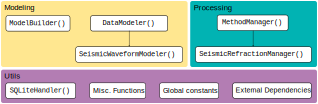
\includegraphics[width=.75\textwidth]{figures/package_structure}
	\caption{Fundamental use case illustrating the modeling of seismic refraction data within the formikoj ecosystem.}
	\label{fig:scheme}
\end{figure}
The formikoj library provides a well thought out data management concept based on the SQLite database engine that does not require a separate server process \footnote{https://www.sqlite.org/index.html, last accessed on \today}. In particular, the information for each project, such as survey geometry and first break traveltimes, are stored in a SQLite database file. Using such an application file format facilitates the cross-platform design of the formikoj library, and provides fast I/O operations through concise SQL queries. The portability of the application file allows for an easy exchange of projects between partners across institutions relying on different IT infrastructures. Accordingly, the formikoj library aims at providing a transparent and customizable framework for the collaborative design of reproducible workflows. The comprehensive usage of clear error and log messages aims at supporting the user throughout the modeling and processing workflows. A meticulous exception handling ensures that the data stored in the SQLite project database is not corrupted in case of erroneous input. Moreover, documenting the user input and the respective responses of the formikoj library with the python logging module provides a timestamped command history that further enhances the transparency and repeatability of the conducted workflows.

We present the application of the formikoj library for the modeling and processing of seismic refraction data based on the fundamental use cases presented in Figure~\ref{fig:modworkflow} and Figure~\ref{fig:procworkflow}, respectively.
\begin{figure}
	\centering
	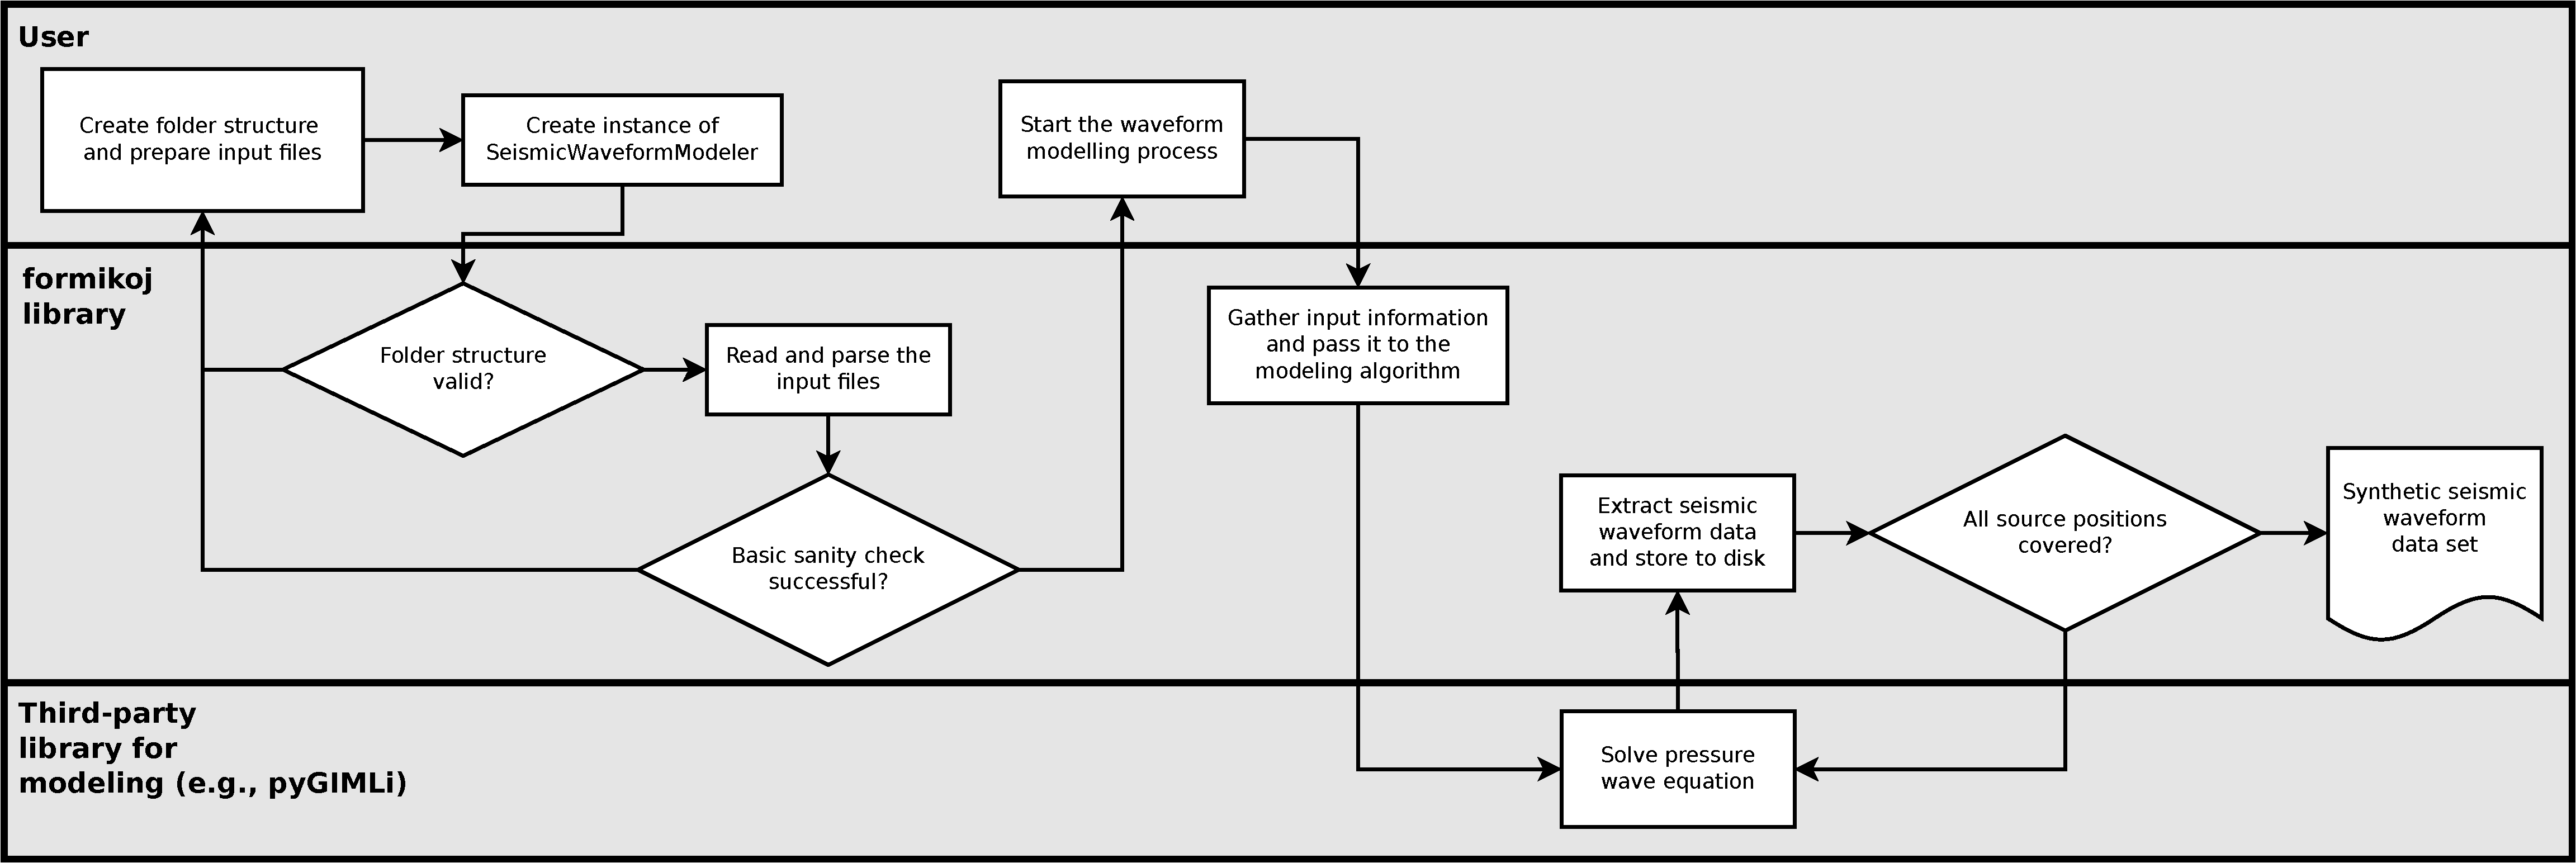
\includegraphics[width=\textwidth]{figures/workflow_modeling-crop.pdf}
	\caption{Fundamental use case illustrating the processing of seismic refraction data within the formikoj ecosystem.}
	\label{fig:modworkflow}
\end{figure}
\begin{figure}
	\centering
	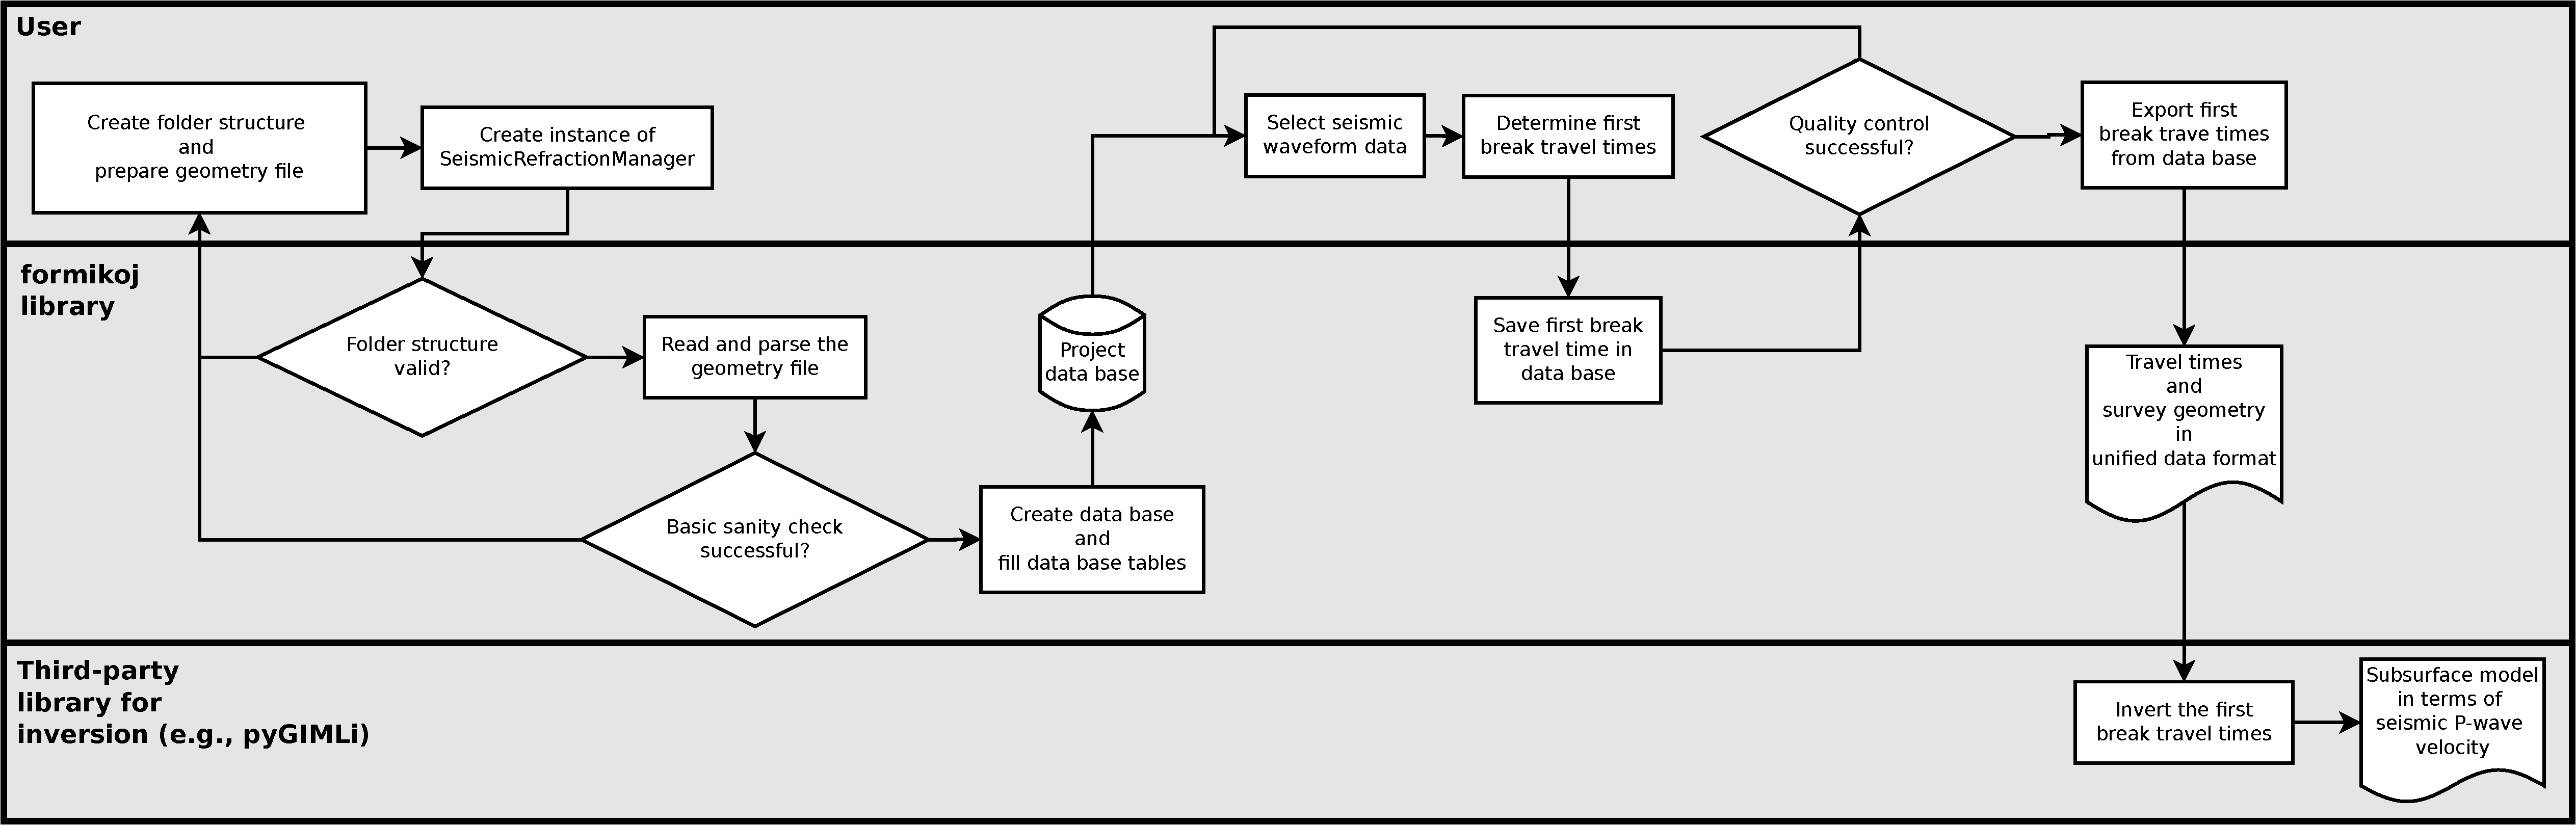
\includegraphics[width=\textwidth]{figures/workflow_processing-crop.pdf}
	\caption{Typical formikoj workflow for the picking of first break traveltimes from seismic waveform data.}
	\label{fig:procworkflow}
\end{figure}
These flow charts illustrate the corresponding workflows as well as the required interactions between the user, the formikoj library and third-party packages. As can be seen from Figure~\ref{fig:modworkflow} and Figure~\ref{fig:procworkflow}, the formikoj library acts as an interface between the user and more complex functionalities of third-party libraries, such as pyGIMLi for modeling and inversion of seismic refraction data.
The \texttt{SeismicWaveformModeler} and \texttt{SeismicRefractionManager} classes implement these fundamental use cases, yet their actual capabilities are continuously expanded, e.g., to address specific modeling or processing requirements as well as to enhance the user experience. To avoid redundancies in the implementation we built these classes upon the functionalities of existing packages such as ObsPy for the processing of seismological data \citep[][]{beyreuther2010} and pyGIMLi for the modeling and inversion of different geophysical data \citep{ruecker2017}. Other important third party dependencies refer to NumPy \citep{harris2020} and Pandas \citep{mckinney2010} for general data handling, as well as matplotlib \citep{hunter2007} and PyVista \citep{sullivan2019} for data visualization.

The formikoj library is primarily developed on machines running Linux Mint \num{20} or Kubuntu \num{22}.\num{04}, respectively. Testing of the library refers to carrying out the fundamental use cases for modeling and processing of seismic refraction data presented in Figure~\ref{fig:modworkflow} and \ref{fig:procworkflow}. To ensure the cross-platform applicability of the formikoj library we test these fundamental use cases also on machines running on Windows \num{10}, Windows \num{11} as well as macOS versions \num{12} and \num{13}.

\subsection{Generation of seismic waveform data for synthetic subsurface models}

The SR method exploits the ground motion recorded by sensors installed in the surface (e.g., geophones) to characterize the propagation of seismic waves generated at well known locations (i.e., shot stations). 
The visualization of the ground motion as function of time yields a so-called seismogram for each geophone position.
Accordingly, the \texttt{SeismicWaveformModeler} class provides a flexible way to generate synthetic seismic waveform data for P-wave refraction modeling either in a python script, interactively in a jupyter notebook or an ipython shell.
To create an instance of the class the user provides the absolute or relative path to the working directory as parameter to the constructor:
\begin{lstlisting}[language=Python]
# Import the SeismicWaveformModeler from the formikoj library
from formikoj import SeismicWaveformModeler

# Create an instance of the SeismicWaveformModeler
swm = SeismicWaveformModeler('.')

\end{lstlisting}

\begin{footnotesize}
\begin{verbatim}
INFO    : Created instance of SeismicWaveformModeler
\end{verbatim}
\end{footnotesize}

In the working directory, the required input files are provided via the subdirectory \textit{in}, whereas the modeling output will be stored in the automatically created subdirectory \textit{out}. The key input file is the measurement scheme as it contains information regarding the distribution of the shot and geophone stations. If provided in the unified data format, the measurement scheme is imported directly with pyGIMLi into a \texttt{DataContainer}. In case the measurement scheme is provided as a csv file, the \texttt{SeismicWaveformModeler} reads the information and writes it to a pyGIMLi \texttt{DataContainer} object. If provided as csv file, the measurement scheme contains a single line for each station in the survey layout, where a station either hosts a geophone or a shot, or both (see Table~\ref{tab:scheme}). The values provided in each line need to be separated by a unique delimiter, and the file must not contain a header.
\begin{table}%[pos=h]
    \caption{Description of the information to be provided in the columns of a measurement scheme in csv format.}
    \centering
    \begin{tabular}{clcl}
        \toprule
        Column & \textbf{Content} & \textbf{Data type} & \textbf{Description} \\
        \midrule
        1 & x coordinate & float & Station x coordinate, e.g., given in (m) \\ 
        2 & y coordinate & float & Station y coordinate, e.g., given in (m) \\ 
        3 & z coordinate & float & Station z coordinate, e.g., given in (m) \\ 
        4 & Geophone & bool & 1 in case of a receiver station, 0 otherwise \\ 
        5 & Shot & bool & 1 in case of a shot station, 0 otherwise \\
        \bottomrule
    \end{tabular}
    \label{tab:scheme}
\end{table}

For the modeling of the seismic waveform data, the parameters characterizing the base wavelet, the synthetic subsurface model and the resulting waveform datasets are provided (see Table~\ref{tab:config}) in a configuration file following the yaml format:

\begin{footnotesize}
\begin{verbatim}
wavelet:
    length: 1.024
    frequency: 100
    sampling_rate: 2000
    pretrigger: 0.02

model:
    velmap: [[1, 750], [2, 2500], [3, 4000]]
    layers: [[1, 3], [2, 5], [3, 15]]
    quality: 32
    area: 10
    smooth: [1, 10]
    sec_nodes: 3    

dataset:
    number: 1
    names: [syn_data]
    noise: 1
    noise_level: 1e-4
    missing_shots: 1
    broken_geophones: 1
    wrong_polarity: 1
    
traveltimes:
    noise_relative: 0.
    noise_absolute: 0.
\end{verbatim}
\end{footnotesize}

In this exemplary configuration, the first block (\texttt{wavelet}) contains the parameterization of the base wavelet, which controls the modeling of the seismic waveforms (see Table~\ref{tab:config}).
The second block (\texttt{model}) contains information regarding the synthetic subsurface model. Here, the user can define simple models with all layers considered to be parallel to the surface topography, which is inferred from the station geometry provided in the measurement scheme. The seismic velocity values for the different model regions (\texttt{velmap}) and the corresponding thickness of the different geological units (\texttt{layers}) have to be explicitly defined in the configuration file. The remaining parameters (\texttt{quality}, \texttt{area}, \texttt{smooth} and \texttt{sec\_nodes}) refer to the properties of the mesh that is eventually used for the forward modeling of the seismic waveform data and corresponding first break traveltimes (we refer to the respective pyGIMLi resources\footnote{https://www.pygimli.org/pygimliapi/\_generated/pygimli.meshtools.html\#pygimli.meshtools.createMesh, last accessed \today} for further information).
In the third block of the exemplary configuration file (\texttt{dataset}), the user can set specific names for the datasets to be created (the number of datasets is automatically determined), or set the number of datasets to be created and the dataset names are automatically generated with the prefix \textit{dataset\_}.
The remaining parameters provided in the \texttt{dataset} block control the random error (\texttt{noise} and \texttt{noise\_level}) as well as systematic errors (\texttt{missing\_shots}, \texttt{broken\_geophones} and \texttt{wrong\_polarity}) in the modeled seismic waveform data (see Table~\ref{tab:config} for a detailed description).
The number and position of the shot and geophone stations affected by the systematic errors are randomly chosen with a maximum of \qty{5}{\%} of the total number of stations in order to avoid a high number of invalid trace data.
The final block of the configuration file (\texttt{traveltimes}) contains data-error parameters for both the absolute error ($e_{abs}$) and the relative error ($e_{rel}$) defined by the user. The data error model is then estimated as

\begin{equation}
	\vecmat{e} = e_{abs} + \vecmat{d}\,e_{rel}\,, 
	\label{eq:esterr}
\end{equation}
where $\vecmat{d}$ denotes the forward modeled data not affected by noise, i.e., here the first break traveltimes obtained through the Dijkstra algorithm \citep{dijkstra1959}. These computed error values are subsequently added to the data to obtain the noisy data as

\begin{equation}
	\vecmat{d_{noise}}=\vecmat{d}\left(1 + \vecmat{e}\right)\,.
	\label{eq:noisydata}
\end{equation}

\begin{table*}[]
    \caption{Description of the parameters, which can be defined in a configuration file used for the modeling of the synthetic seismic data.}
    \centering
    \begin{tabular*}{\tblwidth}{@{} LCL@{}}
        \toprule
        \textbf{Parameter} & \textbf{Unit/} & \textbf{Description} \\
         & \textbf{Data type} & \\ 
        \midrule
        \textbf{\texttt{wavelet}} & & \\
         & & \\
        length & s & Length of the base wavelet, which also defines the \\
         & & length of the synthetic seismic waveform data \\ 
        frequency & Hz & Frequency of the base wavelet \\ 
        sampling\_rate & Hz & Defines temporal resolution of the seismic waveforms \\ 
        pretrigger & s & Add buffer to the seismic waveforms before the onset \\
         & & of the actual data \\
        \midrule
        \textbf{\texttt{dataset}} & & \\
         & & \\
        number & int & Number of datasets to be created \\
        names & list (string) & Names of the datasets \\
        noise & bool & 1 in case noise should be added to the synthetic \\
         & & waveforms, 0 otherwise \\
        noise\_level & - & Level of the seismic background noise \\
        missing\_shots & bool & 1 in case the datasets should be affected by missing \\
         & & shot files, 0 otherwise \\
        broken\_geophones & bool & 1 in case the datasets should comprise broken \\
         & & geophones (i.e., no data in the corresponding \\
         & & seismograms), 0 otherwise \\
        wrong\_polarity & bool & 1 in case the datasets should contain traces with \\
         & & inverse polarity, 0 otherwise \\
        \midrule
        \textbf{\texttt{model}} & & \\
         & & \\
        velmap & list & For each layer the first value defines the marker and \\
         & (float/int) & the second one the seismic velocity within the layer \\
        layers & list & For each layer the first value defines the marker and \\
         & (float/int) & the second one the thickness \\
        \midrule
        \textbf{\texttt{traveltimes}} & & \\
         & & \\
        noise\_relative & \%/100 & Relative noise to be added to the forward modeled \\
      	 & & seismic traveltimes \\
        noise\_absolute & s & Absolute noise to be added to the forward modeled \\
         & & seismic traveltimes\\
        \bottomrule
    \end{tabular*}
    \label{tab:config}
\end{table*}

The configuration file needs to be provided via the input directory from where it can be imported through the \texttt{load} method of the \texttt{SeismicWaveformModeler}:
\begin{lstlisting}[language=Python, firstnumber=6]
# Load and parse the configuration file
swm.load(type='config')
\end{lstlisting}
\begin{footnotesize}
\begin{verbatim}
INFO    : Configuration loaded
\end{verbatim}
\end{footnotesize}
To demonstrate the ability to model seismic waveform data for arbitrary subsurface conditions we do not define a simple subsurface model in the configuration file but provide a more complex model in the binary mesh format (e.g., a bms file). We prepare the model and the corresponding forward modeling mesh based on the mesh tools provided by pyGIMLi and save the mesh in the bms format (a commented version of the corresponding python script can be found in the Appendix). Similar to the configuration file, a bms file stored in the input directory can be imported into the workflow through the \texttt{load} method as follows:
\begin{lstlisting}[language=Python, firstnumber=8]
# Load the mesh into the workflow
swm.load(type='mesh')
\end{lstlisting}
\begin{footnotesize}
\begin{verbatim}
INFO    : Mesh loaded
\end{verbatim}
\end{footnotesize}
The forward modeling process generating the seismic waveform data is then invoked through the \texttt{create} method:
\begin{lstlisting}[language=Python, firstnumber=10]
# Start the modeling of the seismic waveform data
swm.create(type='waveforms')
\end{lstlisting}
\begin{footnotesize}
\begin{verbatim}
INFO    : Measurement scheme loaded
INFO    : Velocity model created
INFO    : Wavelet created
[++++++++++++++ 100% ++++++++++++++] 2048 of 2048 complete
      ...
[++++++++++++++ 100% ++++++++++++++] 2048 of 2048 complete
INFO    : Dataset 'syn\_data' created
\end{verbatim}
\end{footnotesize}
As can be seen from the log messages, the \texttt{SeismicWaveformModeler} first loads the measurement scheme into the workflow. In the second step, the provided mesh and the seismic velocity values defined in the configuration file are combined to create the seismic velocity model considered for the waveform modeling in this study (see Figure~\ref{fig:syndataexample}a). The model consists of a top and a bottom layer with varying thickness characterized by seismic velocity values of \qty{750}{ms^{-1}} and \qty{4000}{ms^{-1}}, respectively. In the center, the model contains an irregularly shaped anomaly associated with a seismic velocity of \qty{2500}{ms^{-1}}, i.e., the model features vertical and lateral variations in the seismic velocity distribution.
\begin{figure}
	\centering
	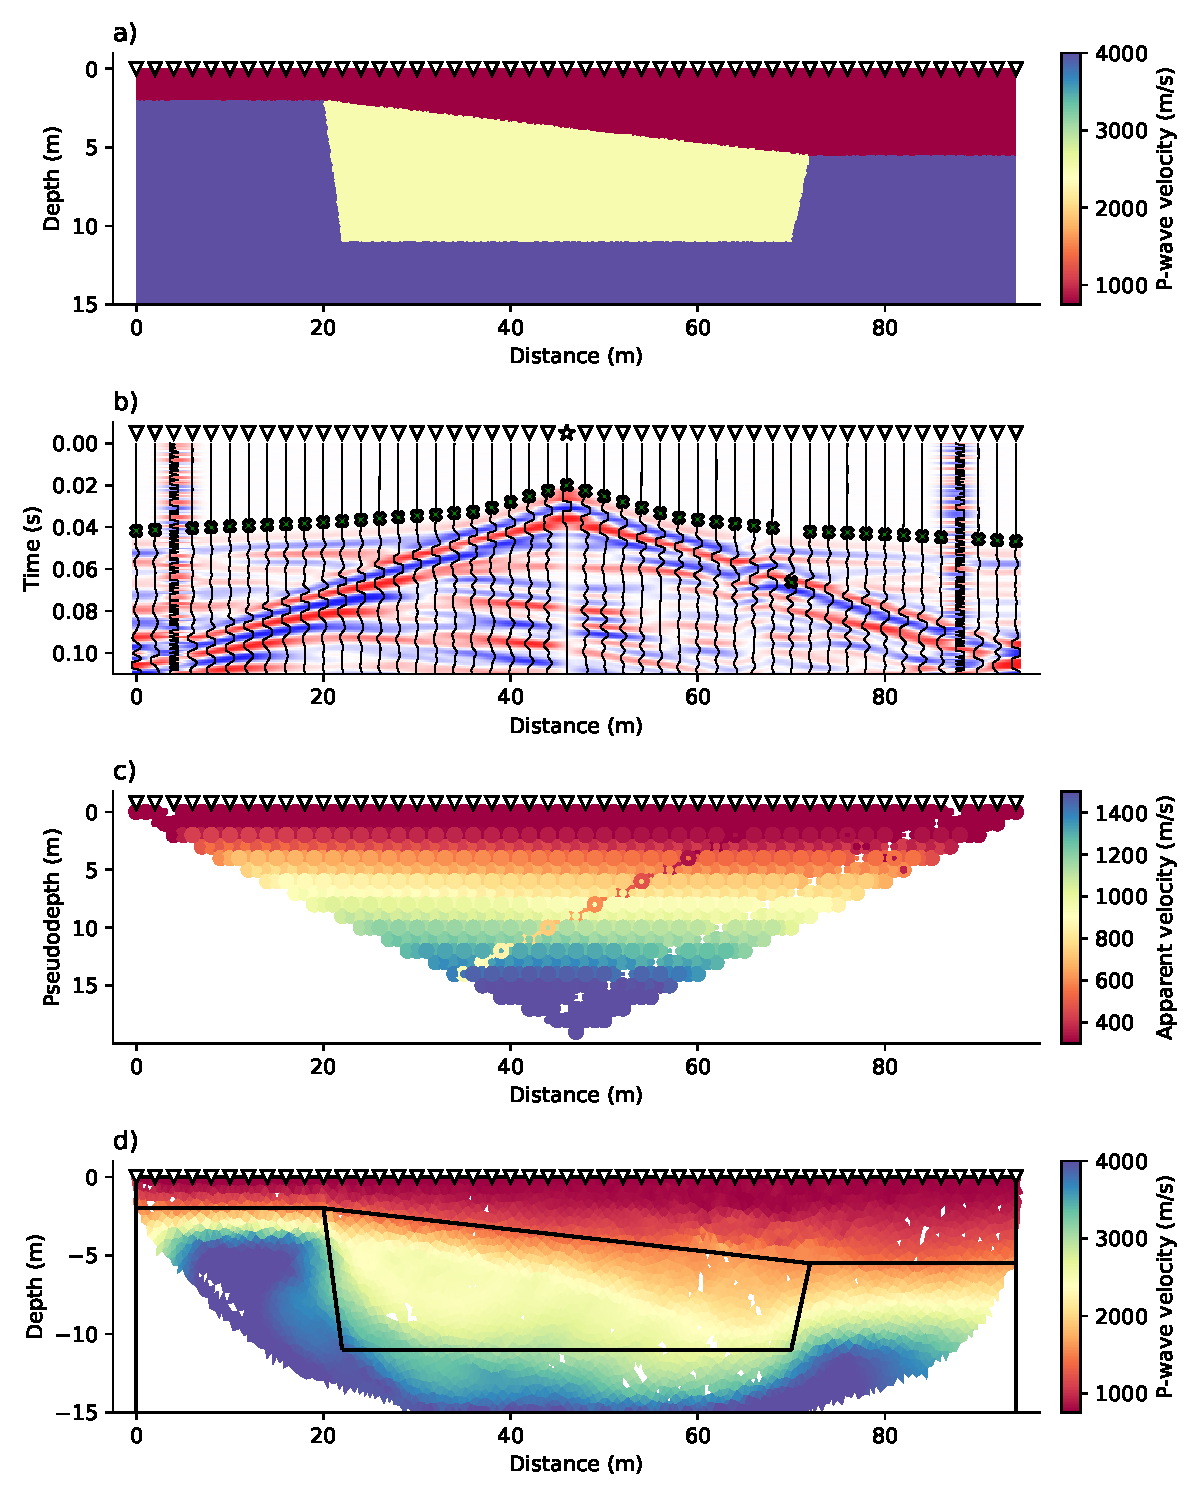
\includegraphics[width=.75\textwidth]{figures/synthetic_data_example.pdf}
	\caption{Synthetic seismic data generated with the \texttt{SeismicWaveformModeler}: \\(a) Two-layered subsurface model without topography characterized by a distinct anomaly in the center. Triangles along the surface indicate the positions of geophones. \\(b) Synthetic seismic waveform data computed from the subsurface model for a shot point (star-shaped symbol) located in the center of the profile. \\(c) Pseudosection illustrating the apparent velocity computed from the seismic traveltimes based on the survey geometry. \\(d) Subsurface model of the seismic P-wave velocity distribution obtained through the inversion of the synthetic P-wave traveltimes.}
	\label{fig:syndataexample}
\end{figure}
The third step refers to the generation of a Ricker wavelet through the pyGIMLi function \texttt{ricker} as

\begin{equation}
	u = \left(1-2\pi^2f^2t^2\right)e^{-\pi^2f^2\left(t-t_0\right)^2}\,
	\label{eq:ricker}
\end{equation}
based on the wavelet properties provided in the configuration file. In Equation~\ref{eq:ricker}, $f$ is the frequency of the wavelet given in \unit{Hz}, $t$ refers to the time base definition, i.e., the length and resolution of the wavelet in the time domain, and $t_0$ is the time offset of the wavelet.

Based on the mesh, the velocity model and the Ricker wavelet we use pyGIMLi 
to solve the pressure wave equation for each shot station defined in the measurement scheme.
The resultant seismograms are extracted at the corresponding geophone stations, gathered for each shot position in an ObsPy \texttt{Stream} object and saved in the output directory (\textit{out}) as shown here:
\dirtree{%
.1 working\_directory.
.2 in.
.2 out.
.3 syn\_data.
.4 data.
.5 protocol.txt.
.5 station\_coords.csv.
.5 Shot\_1001.syn.
.5 ....
.5 Shot\_10nn.syn.
.4 syn\_data\_tt.pck.
.4 info.txt.
}
In particular, the subdirectory \textit{data} contains a separate file in the miniseed format \citep{ahern2012, ringler2015} for each shot position, where the file extension \textit{syn} indicates that the shot files contain forward modeled seismic waveform data. 
The measurement protocol (protocol.txt) and the station coordinates provided as a csv file (station\_coords.csv) are also stored in this directory. The header of the measurement protocol contains the survey parameters, e.g., sampling rate, recording length, number of geophones and geophone spacing. Moreover, the protocol associates each shot file of the dataset with a specific location in the survey geometry with respect to the geophone positions, e.g.:
\begin{footnotesize}
\begin{verbatim}
 #############################
   Line: SYN_syn_data             
   Sampling rate: 2000 Hz    
   Recording length: 0.512 s 
   Number of geophones: 48   
   Geophone spacing: 2 m     
 #############################
 
     File number | Station
         1001    |   G001
           :     |     :
         1048    |   G048
\end{verbatim}
\end{footnotesize}
The auxiliary file info.txt exported to the dataset directory summarizes the parameters from the configuration file as well as information regarding the simulated systematic errors in the synthetic seismic waveform data, e.g.:
\begin{footnotesize}
\begin{verbatim}
Number of geophones: 48
Number of shots: 48
Recording length (s): 0.512
Sampling frequency (Hz): 2000
Wavelet type: Ricker
Frequency of the wavelet (Hz): 100

Missing shot(s): 11
Broken geophone(s): 13
Wrong polarity geophone(s): 26
\end{verbatim}
\end{footnotesize}

Figure~\ref{fig:syndataexample}b presents the seismic waveform data forward modeled for a shot point located in the center of the profile. The seismograms are shown as curves, whereas the strength of the amplitudes is added as color-coded information. In the seismograms we see clear first onsets along the entire profile, yet receivers 3 and 45 were modeled as broken geophones, i.e., the corresponding seismograms contain solely noise. Crosses overlaid on the valid seismograms at the respective first onset indicate the first break traveltimes $tt$ between the shot and the receiver. In addition to the missing first break traveltimes for the broken receivers, we manually added a systematic error, i.e., we set an erroneous traveltime for receiver 36, to demonstrate how such outliers can be identified in a so-called pseudosection.

Pseudosections are a useful tool for the analysis of the data quality by presenting the data based on the positions of shots and receivers. Such a visualization allows for the detection of outliers and their spatial distribution as necessary to understand possible sources of error. In case of the SRT, a pseudosection as presented in Figure~\ref{fig:syndataexample}c, illustrates apparent velocity ($v_{app}$) values computed as

\begin{equation}
	v_{app}=\frac{aoffset}{tt}\,,
	\label{eq:vapp}
\end{equation}
where $aoffset$ refers to the absolute offset between shot and receiver. The $v_{app}$ values are plotted at pseudolocations, where the location along profile direction is defined by the midpoint of the corresponding shot-receiver pair and the pseudodepth is computed as $1/3$ of $aoffset$.
As demonstrated in Figure~\ref{fig:syndataexample}c, a pseudosection allows for the identification of missing data (e.g., receiver 3 and 45) as well as systematic errors or outliers, i.e., velocities erroneously influenced by a single shot or receiver (see receiver 36). The main assumption here is that the pseudosection should reveal smooth transitions between lateral and vertical neighbors, considering that the data were collected with gradual changes in the position of the source (i.e., hammer blow) and the receiver (i.e., geophone). The pseudosection will reveal large variations in case of abrupt changes in the topography or the geometry of the array, yet this can be taken into account by the user during the identification of outliers and possible systematic errors.

Based on pseudosections erroneous traveltimes can be identified and subsequently removed or corrected, which is a critical processing step prior to the inversion of the data. The inversion of first break traveltimes aims at resolving a model of the P-wave velocity of the subsurface materials, where systematic errors in the data would lead to the creation of artifacts in the imaging results or hinder the convergence of the inversion.
Considering the multitude of available inversion frameworks we do not include a new inversion strategy in the formikoj library. Instead the processed data can be exported in any format required for the use of commercial inversion algorithms, or can be linked directly to other open-source libraries. In our case, we refer to the modeling and inversion capabilities of pyGIMLi \citep{ruecker2017}.
pyGIMLi uses a generalized Gauss-Newton method to solve the inversion problem through the minimization of an objective function given as:

\begin{equation}
	\parallel\vecmat{W}_d\left(\mathcal{F}\left(\vecmat{m}\right)-\vecmat{d}\right)\parallel_2^2+\lambda\parallel\vecmat{W}_m\left(\vecmat{m}-\vecmat{m}_0\right)\parallel_2^2\rightarrow\textrm{min}
	\label{eq:objfct}
\end{equation}
The first term on the right-hand side of Equation~\ref{eq:objfct} refers to the data misfit. $\vecmat{W}_d$ is the data weighting matrix holding the reciprocals of the data errors, $\vecmat{d}$ denotes the data vector holding the input data (first break traveltimes), $\vecmat{m}$ is the model vector representing the target parameter (seismic P-wave velocity values), and $\mathcal{F}\left(\vecmat{m}\right)$ is the model response.
The second term denotes represents the regularization, where $\vecmat{W}_m$ and $\vecmat{m}_0$ are the model constraint matrix and the reference model, respectively. The regularization parameter $\lambda$ balances the influence of the data misfit and the regularization term on the inversion process.

The inversion of the synthetic first break traveltimes considered here resolves the subsurface model presented in Figure~\ref{fig:syndataexample}d, which is given in terms of the spatial variations of the seismic P-wave velocity, i.e., reflecting the associated lateral and vertical variations. Depending on the survey geometry the inversion can resolve subsurface models in both 2D or 3D. 
To aid in the evaluation of this inversion result we superimposed the known interfaces between the different subsurface unit of the synthetic model. As can be seen from this plot, the imaging result resolves the fundamental structural features  and reflects the P-wave velocity distribution of the synthetic subsurface model. Deviations from the true velocity model are due to the smoothness-constraint inversion scheme applied by pyGIMLi. To obtain sharper contrasts between the different subsurface units in the imaging result structural constraints could be incorporated in the inversion, e.g., as demonstrated by \citep{steiner2021}; yet, the exploration of different inversion strategies is beyond the scope of this study. We consider Figure~\ref{fig:syndataexample} to demonstrate the applicability of the \texttt{SeismicWaveformModeler} class for generating synthetic seismic waveform data to be used in numerical P-wave refraction seismic investigations.

\subsection{Processing of seismic refraction datasets}

The seismic refraction (SR) method is based on the measurement of the traveltimes of seismic waves determined from the the first onset of the seismic energy recorded by geophones. In the SRT, the inversion of traveltimes gathered from tens to hundreds of seismograms permits the computation of variations in the seismic velocities in an imaging framework. Measuring the traveltimes in seismograms (i.e., first break picking) is commonly done manually (or semi-automatically) in an iterative process. The signal-to-noise ratio in the recorded seismograms substantially influences the quality of the traveltimes picked in the seismograms, and thus the seismic velocity model obtained through the inversion. Accordingly, a proper enhancement of the perceptibility of the first onsets is crucial.

The \texttt{SeismicRefractionManager} class provides functionalities that permit the processing of seismic waveform data for a refraction seismic analysis. These functionalities involve the reading of seismic waveform data, combining the data with information about the survey geometry, processing of the waveforms as well as the picking of first break traveltimes. Since the first break picking is a highly interactive process, the \texttt{SeismicRefractionManager} is designed primarily for usage from within an ipython shell. The first break traveltimes determined with the\\ \texttt{SeismicRefractionManager} represent the input data, e.g., for the \texttt{TravelTimeManager} of pyGIMLi \citep{ruecker2017}. This is particularly relevant as the \texttt{TravelTimeManager} provides an inversion framework for first break traveltimes, yet not a framework for the processing of seismic waveform data.
For the demonstration of the fundamental \texttt{SeismicRefractionManager} capabilities we consider the synthetic seismic data created with the\\ \texttt{SeismicWaveformModeler} above, which illustrates that both classes can be combined in subsequent workflows. 

\subsubsection{Compiling the survey information and creating a project}

To create a new or load an existing \texttt{SeismicRefractionManager} project, the working directory needs to contain specific subdirectories:

\dirtree{%
.1 working\_directory.
.2 01\_data.
.3 raw.
.2 02\_geom.
.2 03\_proc.
}
In this directory structure, the seismic shot files are stored in \textit{01\_data/raw} and the geometry file (\textit{geometry.csv}) is provided in \textit{02\_geom}.
The geometry file is a csv file that provides an abstract representation of the survey layout and must not contain a header. The fundamental element for the description of the survey layout is the station, which refers either to a geophone position, a shot position or a position with co-located shot and geophone. For each station the geometric and semantic information described in Table~\ref{tab:geometry} are provided column-wise, i.e., each line in the geometry file corresponds to a single station with a unique position within the survey layout. 
\begin{table}[pos=h]
    \caption{Description of the information to be provided in the columns of the geometry file.}
    \centering
    \begin{tabular}{clcl}
        \toprule
        \textbf{Col} & \textbf{Content} & \textbf{Data type} & \textbf{Description} \\
        \midrule
        1 & x coordinate & float & Station x coordinate, e.g., given in (m) \\ 
        2 & y coordinate & float & Station y coordinate, e.g., given in (m) \\ 
        3 & z coordinate & float & Station z coordinate, e.g., given in (m) \\ 
        4 & Geophone & bool & 1 if a geophone was deployed at station, 0 otherwise \\ 
        5 & Shot & int & The numerical part of the file name, e.g., 1001, if a shot was conducted \\
          & & & at this station, -1 otherwise \\ 
        6 & First geophone & int & First active geophone (-1 if no shot was conducted at the station) \\ 
        7 & Number of geophones & int & Number of active geophones (-1 if no shot was conducted at the station) \\
        \bottomrule
    \end{tabular}
    \label{tab:geometry}
\end{table}
For the synthetic dataset considered in this study, the 2D station coordinates are provided in the geometry file, whereas the z coordinate is assumed to be \qty{0}{m} along the entire profile, as illustrated in Table~\ref{tab:syn_geometry}; thus, reflecting the lack of surface topography in the synthetic model (see Figure~\ref{fig:syndataexample}a). In the column \textbf{Geo} the geometry file contains the value 1 (True) for each station except the station located at \qty{24}{m} referring to the broken geophone modeled by the \texttt{SeismicWaveformModeler}. When compiling the geometry file we also need to take into account the missing shot at station 11, i.e., the station located at \qty{20}{m} along profile direction, and set the corresponding value to \num{-1}. 
The column \textbf{1st Geo} indicates the first active geophone along the profile for each shot file, which for the synthetic dataset considered here is the geophone deployed at the first station along the entire profile. In particular, the column \textbf{1st Geo} allows the reproduction of roll-along survey geometries, where in the first segment the first active geophone is always the geophone at station 1. Considering 48 geophones deployed in each segment, and an overlap of \qty{50}{\%}, the first geophone for the consecutive segments would be 25, 49, 73, 97, and so on. 
\begin{table}
   \caption{Excerpt from the geometry file describing the survey geometry of the synthetic dataset generated in this study.}
    \centering
    \begin{tabular}{rrrcrrr}
        \toprule
        \textbf{x (m)} & \textbf{y (m)} & \textbf{z (m)} & \textbf{Geo} & \textbf{Shot} & \textbf{1st Geo} & \textbf{\# Geo} \\
        \midrule
		0.0 & 0.0 & 0.0 & 1 & 1001 & 1 & 48 \\
		2.0 & 0.0 & 0.0 & 1 & 1002 & 1 & 48 \\
        \vdots & \vdots & \vdots & \vdots & \vdots & \vdots & \vdots \\
		20.0 & 0.0 & 0.0 & 1 & -1 & 1 & 48 \\
        \vdots & \vdots & \vdots & \vdots & \vdots & \vdots & \vdots \\
        24.0 & 0.0 & 0.0 & 0 & 1013 & 1 & 48 \\
        \vdots & \vdots & \vdots & \vdots & \vdots & \vdots & \vdots \\
		92.0 & 0.0 & 0.0 & 1 & 1047 & 1 & 48 \\
		94.0 & 0.0 & 0.0 & 1 & 1048 & 1 & 48 \\
        \bottomrule
    \end{tabular}
    \label{tab:syn_geometry}
\end{table}

An instance of the \texttt{SeismicRefractionManager} can be created by providing the path to the working directory as parameter to the constructor. Depending on the content of the working directory, the \texttt{SeismicRefractionManager} automatically decides whether (i) to start in the data preview mode (first break picking not possible), (ii) create a new project, or (iii) load an existing project from disk.
In case the shot files as well as the geometry file are provided and a basic sanity check of the geometry file was successful, the \texttt{SeismicRefractionManager} creates a new project:
\begin{lstlisting}[language=Python, firstnumber=1]
# Import the SeismicRefractionManager from the formikoj library
from formikoj import SeismicRefractionManager

# Create an instance of the SeismicRefractionManager
srm = SeismicRefractionManager('.')
\end{lstlisting}
\begin{footnotesize}
\begin{verbatim}
INFO    : Read geometry information from file
INFO    : Extracted shot geometry
INFO    : Extracted receiver geometry
INFO    : Applied geometry
INFO    : Standard pickset 'picks' created
INFO    : Pickset 'picks' loaded
INFO    : 'picks' set as active pickset
Progress <==============================> 100.0% completed
INFO    : Read 48 files
\end{verbatim}
\end{footnotesize}
In a first step, the \texttt{SeismicRefractionManager} creates an SQLite database \textit{prj.db} in the working directory based on the entity-relationship diagram shown in Figure~\ref{fig:database}.
\begin{figure}
	\centering
	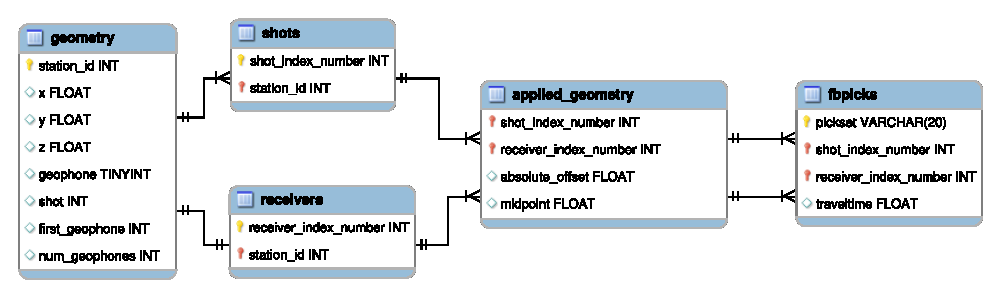
\includegraphics[width=.75\textwidth]{figures/srm_erd.eps}
	\caption{Entity-relationship diagram illustrating the SQLite database used in a \texttt{SeismicRefractionManager} project to store an manage processing related information.}
	\label{fig:database}
\end{figure}
The geometry information is then read from the geometry file and stored in the database table \textit{geometry} with consecutively numbered stations (see Figure~\ref{fig:statnum}). To allow for an efficient data selection for the user the \texttt{SeismicRefractionManager} creates database tables \textit{shots} an d\textit{receivers}, which link the station numbers to shot index numbers (SIN) and receiver index numbers (RIN), respectively. For each shot-receiver pair the corresponding SIN and RIN are stored in the table \textit{applied\_geometry} together with the absolute offset and midpoint between these stations, i.e., the geometry is applied.
In the last step, the database table \textit{fbpicks} is created, which stores the first break traveltimes for each SIN-RIN pair together with the name of the corresponding pickset, i.e., a common label for an entire set of first break traveltimes. By default, each project contains the default pickset 'picks', which is loaded and activated on startup. Once the database is initialized, the waveform data are read from disk and the project is ready for processing.
\begin{figure}
	\centering
	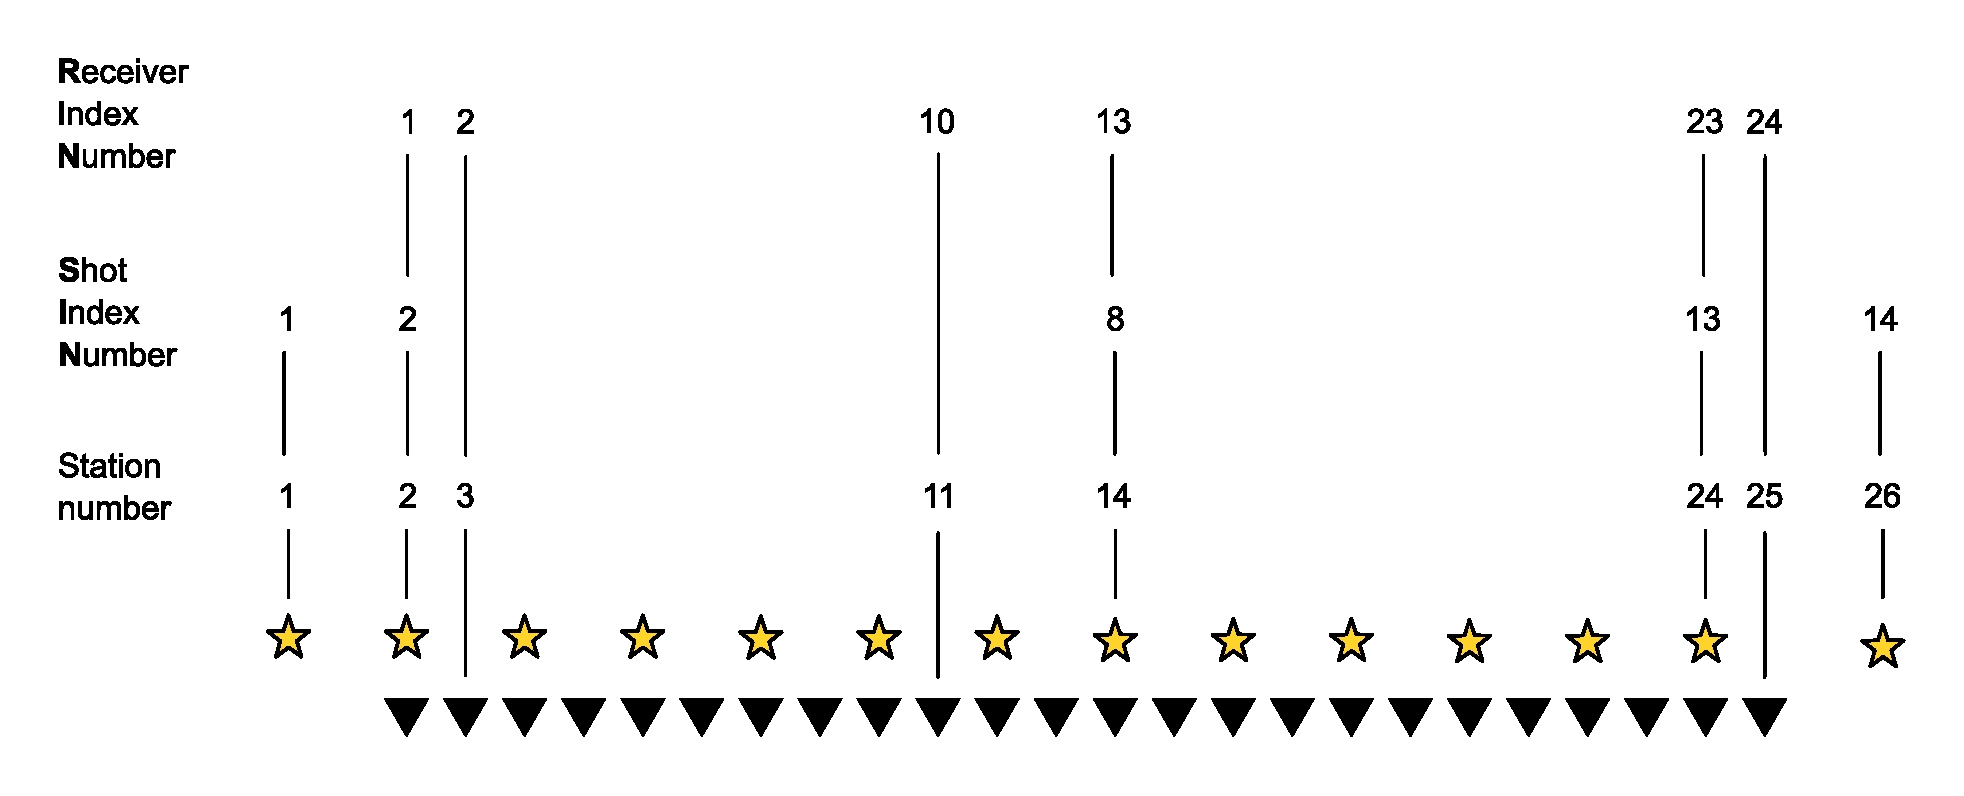
\includegraphics[width=.75\textwidth]{figures/station_numbering.pdf}
	\caption{The \texttt{SeismicRefractionManager} addresses the stations through consecutive station numbers based on the sort order in the geometry file. The shot index numbers (SIN) and receiver index numbers (RIN) are assigned to the shot and receiver stations separately to allow for an intuitive data handling for the user.}
	\label{fig:statnum}
\end{figure}

\subsubsection{Selecting and visualizing seismic waveform data}
Once the geometry is applied the \texttt{select} method of the \texttt{SeismicRefractionManager} allows to gather the seismic waveform data based on a common absolute offset (\texttt{aoffset}), a common RIN (\texttt{rin}), or a common SIN (\texttt{sin})
\begin{lstlisting}[language=Python, firstnumber=6]
# Select traces with common absolute offset
srm.select(by='aoffset', num=6)
\end{lstlisting}
\begin{footnotesize}
\begin{verbatim}
INFO    : 88 traces selected
\end{verbatim}
\end{footnotesize}
\begin{lstlisting}[language=Python, firstnumber=8]
# Select traces with receiver
srm.select(by='rin', num=10)
\end{lstlisting}
\begin{footnotesize}
\begin{verbatim}
INFO    : 48 traces selected
\end{verbatim}
\end{footnotesize}
\begin{lstlisting}[language=Python, firstnumber=10]
# Select traces with receiver
srm.select(by='sin', num=23)
\end{lstlisting}
\begin{footnotesize}
\begin{verbatim}
INFO    : 48 traces selected
\end{verbatim}
\end{footnotesize}

Figure~\ref{fig:spectrum} shows the frequency spectrum of the currently selected traces, which can be computed and visualized through the \texttt{plot} method:
\begin{lstlisting}[language=Python, firstnumber=12]
# Plot the frequency spectrum
srm.plot(type='spectrum')
\end{lstlisting}
The \texttt{SeismicRefractionManager} resolves the frequency spectrum by computing the stacking the power spectral density ($psd$) of the seismograms $s\left(t\right)$ as

\begin{equation}
	psd=10\log_{10}\left(\frac{\lvert \textrm{fft}\left(s\left(t\right)\right)\rvert^2}{N}\right)\,,
\end{equation}
where $\textrm{fft}$ refers to the fast fourier transformation (FFT) and $N$ is the number of the considered seismograms.
The frequency spectrum provides information regarding the amplitudes associated to different frequencies in the seismograms, which can be use for the identification of the dominating frequencies as required for the selection and application of adequate filters such as lowpass, highpass, bandpass and bandstop implemented in ObsPy \citep{beyreuther2010}.
To enhance the signal-to-noise ratio of the seismograms the user can apply the respective filters through the \texttt{filter} method, which utilizes the frequency filters implemented in the ObsPy package \citep[lowpass, highpass, bandpass and bandstop;][]{beyreuther2010}, e.g.:
\begin{lstlisting}[language=Python, firstnumber=14]
# Apply bandpass filter
srm.filter(type='bandpass', freqmin=10, freqmax=120)
\end{lstlisting}
\begin{footnotesize}
\begin{verbatim}
INFO    : Applied bandpass filter (10.0 to 120.0 Hz)
\end{verbatim}
\end{footnotesize}
\begin{figure}
	\centering
	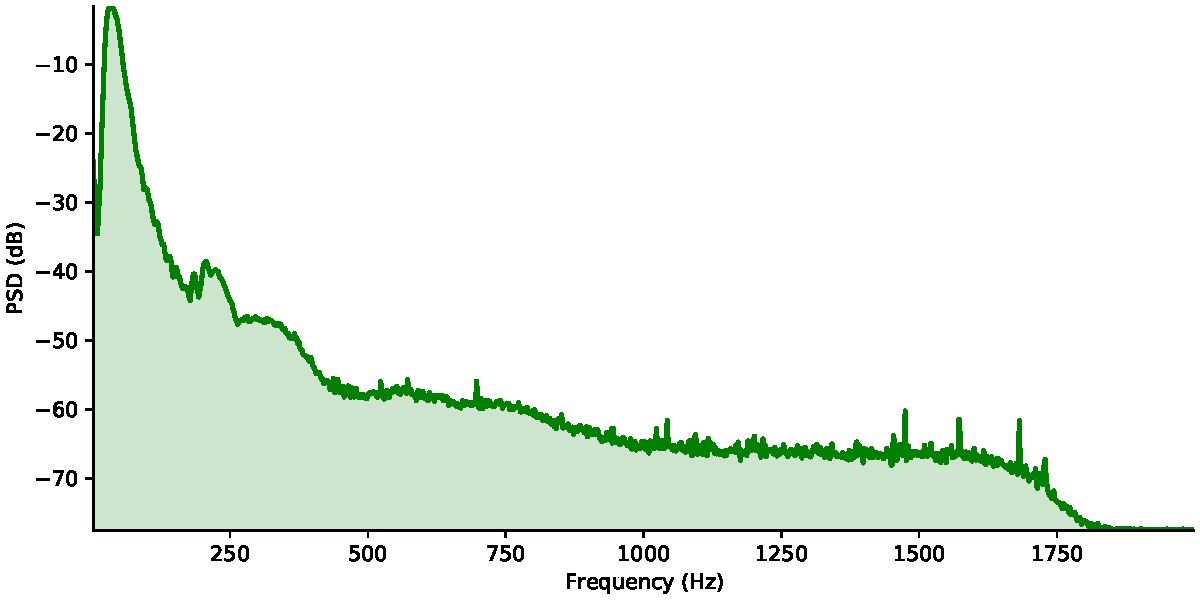
\includegraphics[width=.75\textwidth]{figures/spectrum.pdf}
	\caption{The frequency spectrum illustrates the frequency content of the currently selected traces, which allows for the identification of frequency ranges associated to noise allowing for the definition of corresponding frequency filter settings.}
	\label{fig:spectrum}
\end{figure}
In this example, the filter is solely applied to the currently selected traces, yet setting the parameter \texttt{onhold} as \texttt{True} automatically filters all subsequently selected traces with the same filter settings, e.g.:
\begin{lstlisting}[language=Python, firstnumber=16]
# Apply lowpass filter
srm.filter(type='lowpass', freq=200, onhold=True)
\end{lstlisting}
\begin{footnotesize}
\begin{verbatim}
INFO    : Applied 200.0 Hz lowpass filter
INFO    : Set filter hold on
\end{verbatim}
\end{footnotesize}

The currently selected traces can be visualized by calling the \texttt{plot} method without passing any parameter:
\begin{lstlisting}[language=Python, firstnumber=18]
# Plot selected traces
srm.plot()
\end{lstlisting}
By default, the seismogram plot visualizes the seismic waveforms in a combination of wiggle trace and variable area mode, i.e., the trace data are shown as curves. The area of the curves is colored red for negative and blue for positive amplitudes, respectively (not shown for brevity). Pressing the up or down arrow key on the keyboard toggles between variable area and variable density mode, with the latter reflecting the strength of the amplitudes by the color saturation, i.e., high amplitudes refer to a stronger shade than low amplitudes (see Figure~\ref{fig:srm_intro}).
\begin{figure}
	\centering
	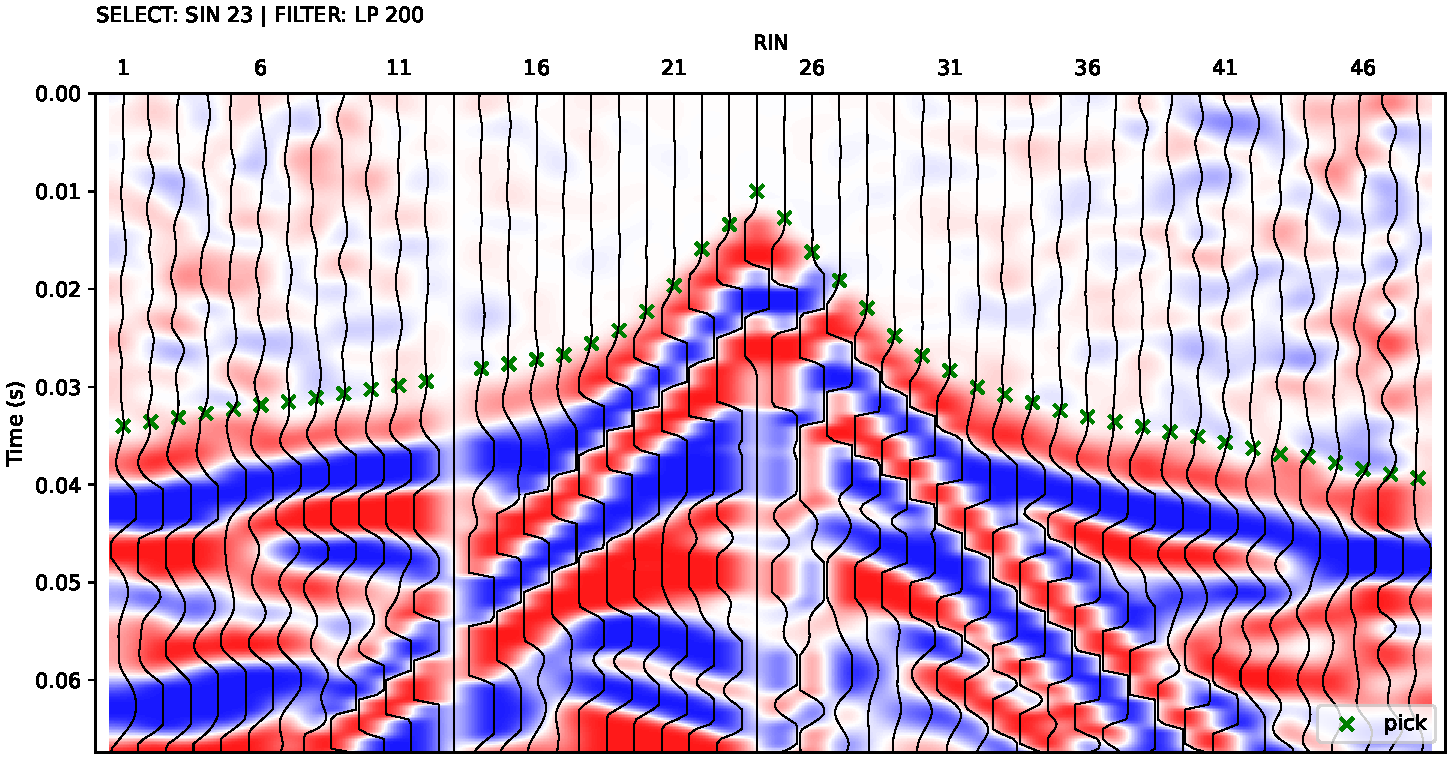
\includegraphics[width=.75\textwidth]{figures/srm_intro.pdf}
	\caption{The seismogram plot presents the currently selected traces along the x axis, where the sort order is determined through the geometry. The corresponding trace data are illustrated as a function of time along the y axis (solid curves), with positive and negative amplitudes depicted in blue and red, respectively. The selection criterion and the applied filter are shown in the upper left corner of the plot. Green crosses refer to the picked traveltimes stored in the currently active pickset.}
	\label{fig:srm_intro}
\end{figure}
The active processing mode and data scaling mode are reported together with the traveltime at the current cursor position in the status bar of the seismogram plot window (see Figure~\ref{fig:statusbar_intro}).
The initial processing mode is 'Fb pick', i.e., first break picking is possible. Additional modes, accessible through the keyboard, allow for an enhanced visualization of the seismograms, e.g., associated to broken geophones or seismograms with wrong polarity. 
The 'm' key activates the trace mute mode ('Trc mute'), which allows to set the amplitude of a trace to zero by clicking with the left mouse button; clicking again on the same trace restores the amplitude information. The trace reverse mode ('Trc rev') is activated by pressing the 'r' key and enables the user to toggle the polarity of a trace by clicking on it with the left mouse button. 
The default data scaling mode is 'Zoom', which allows the scaling of the y-axis by turning the mouse wheel. By pressing the 'a' key the amplitude scaling mode ('Amp scal') is activated. Turning the mouse wheel increases or decreases the amplitudes of the traces currently shown in the seismogram plot, and thus might help to enhance the perceptibility of the first onsets.
By pressing the key of the currently active mode again, the \texttt{SeismicRefractionManager} returns to the default mode; yet, the different modes can be activated in any arbitrary order (as illustrated in Figure~\ref{fig:statusbar_intro}).
\begin{figure}
	\centering
	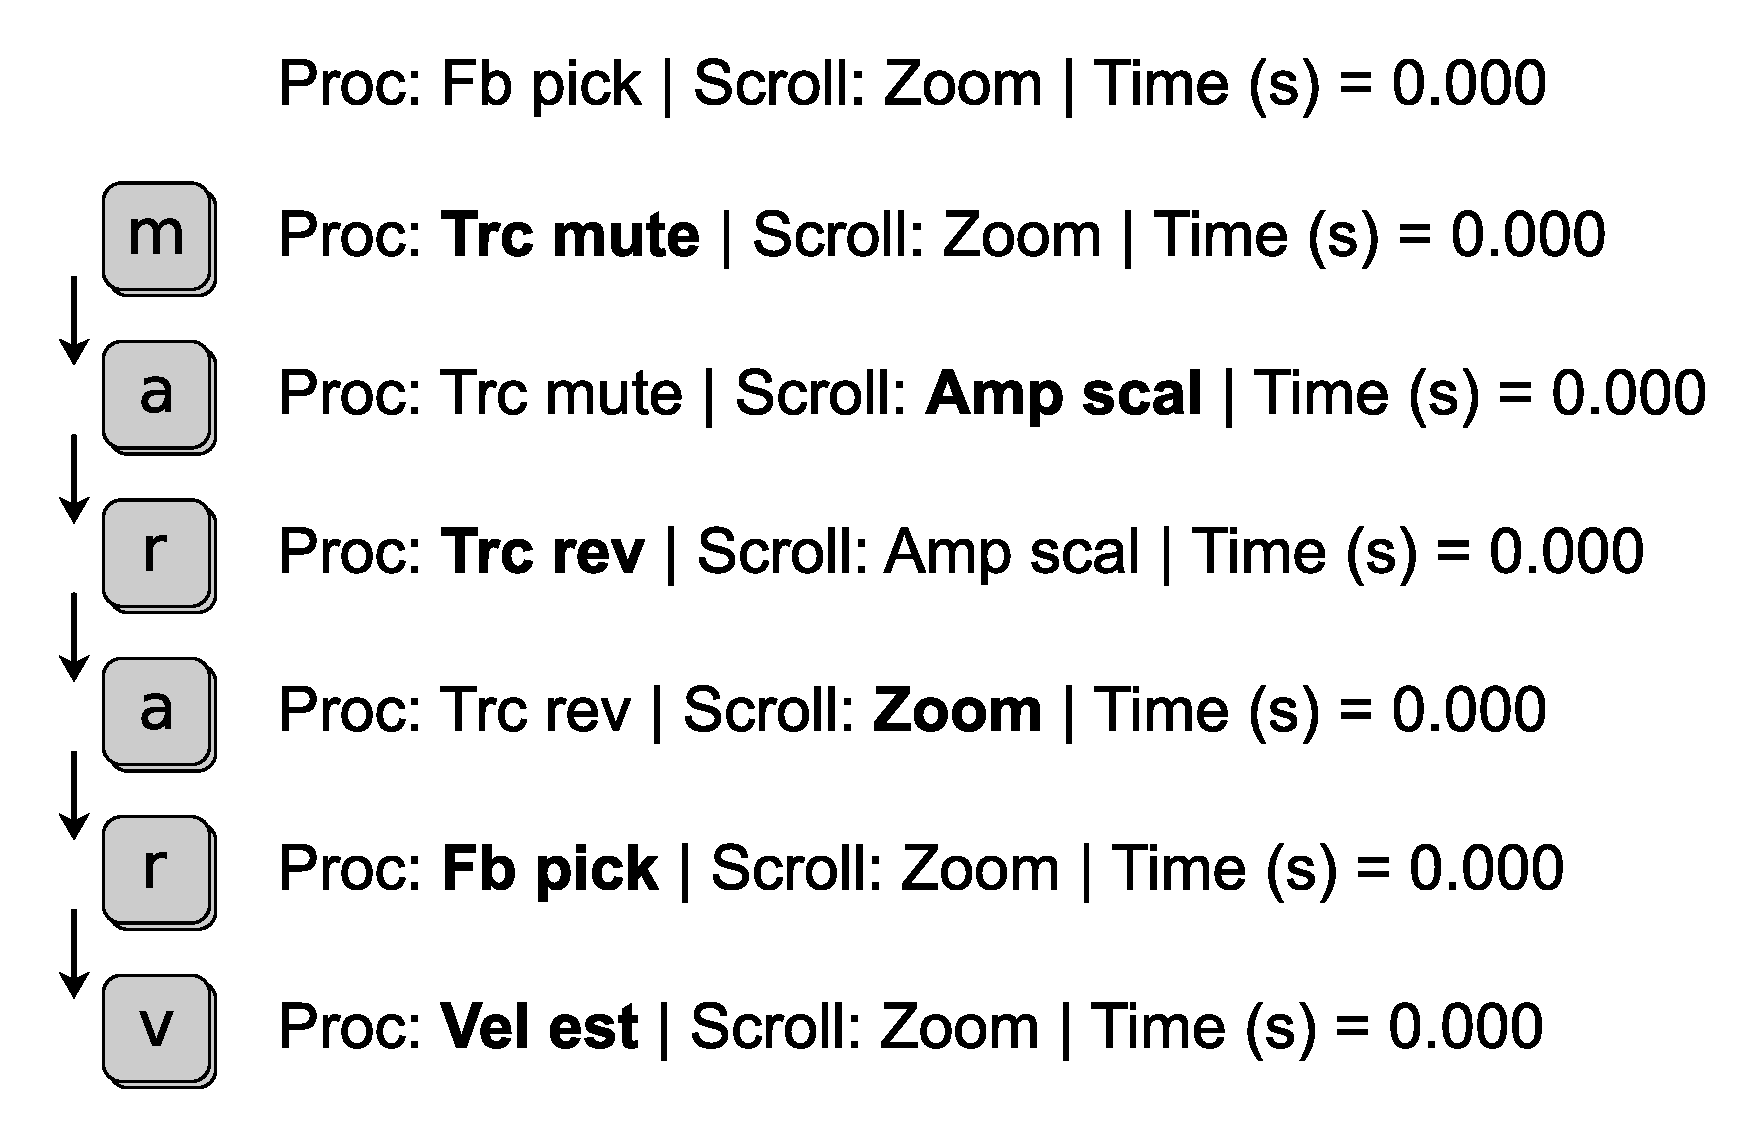
\includegraphics[width=.75\textwidth]{figures/status_bar.pdf}
	\caption{The status bar in the interactive seismogram plot displays the currently active processing and data scaling modes as well as the time (in seconds) at the current cursor position. By pressing the keys 'a', 'm', 'r', 'v' on the keyboard the different modes can be activated.}
	\label{fig:statusbar_intro}
\end{figure}

\subsubsection{Analysis of the seismic waveforms and first break traveltime picking}

In the seismogram plot, the waveforms can be analyzed and processed to obtain information about the subsurface conditions. Activating the velocity estimation mode ('Vel est') by pressing the 'v' key on the keyboard, enables the user to estimate velocities for different wave phases (e.g., originating from a refractor) by pressing the left mouse button and moving the cursor. Once the left mouse button is released, a line between the start and end point is drawn and labeled with the corresponding velocity (estimates can be deleted by clicking with the right mouse button).

If the processing mode 'Fb pick' is activated, picking of first break traveltimes is done individually by clicking with the left mouse button on the respective trace. Clicking again on the same trace will set the first break pick to the new location as there can only be one traveltime for each SIN-RIN pair; whereas clicking with the right mouse button deletes the pick. Alternatively, first break picks can be set for multiple traces by pressing the left mouse button and moving the cursor. 
Once the left mouse button is released, first break picks are defined at the intersections between the line and the seismograms. In the same way, multiple picks can be deleted if a line is drawn with the right mouse button pressed. The first break traveltimes determined in the seismogram plot are automatically written to the project database when the window is closed or another set of traces is loaded by pressing the 'left' or 'right' arrow keys on the keyboard. 

The traveltime diagram for the currently active pickset can be created through the \texttt{plot} method:
\begin{lstlisting}[language=Python, firstnumber=20]
# Plot traveltime diagram
srm.plot(type='traveltimes')
\end{lstlisting}
Figure~\ref{fig:traveltimes_intro} presents an exemplary traveltime diagram, which is a common way to examine the quality of the first break picking. Such illustration of the traveltimes can be used to identify outliers or erroneous measurements, which are commonly associated to traveltimes with substantial deviations from those observed at adjacent stations such as the first break pick for the SIN-RIN pair (23, 11). Outliers can be removed by clicking on the respective data point in the traveltime diagram, which is instantly synchronized with the project database. If the seismogram plot and the traveltime diagram are used side-by-side, changes made to the first break picks in one window will interactively trigger an update of the other one and vice versa.
\begin{figure}
	\centering
	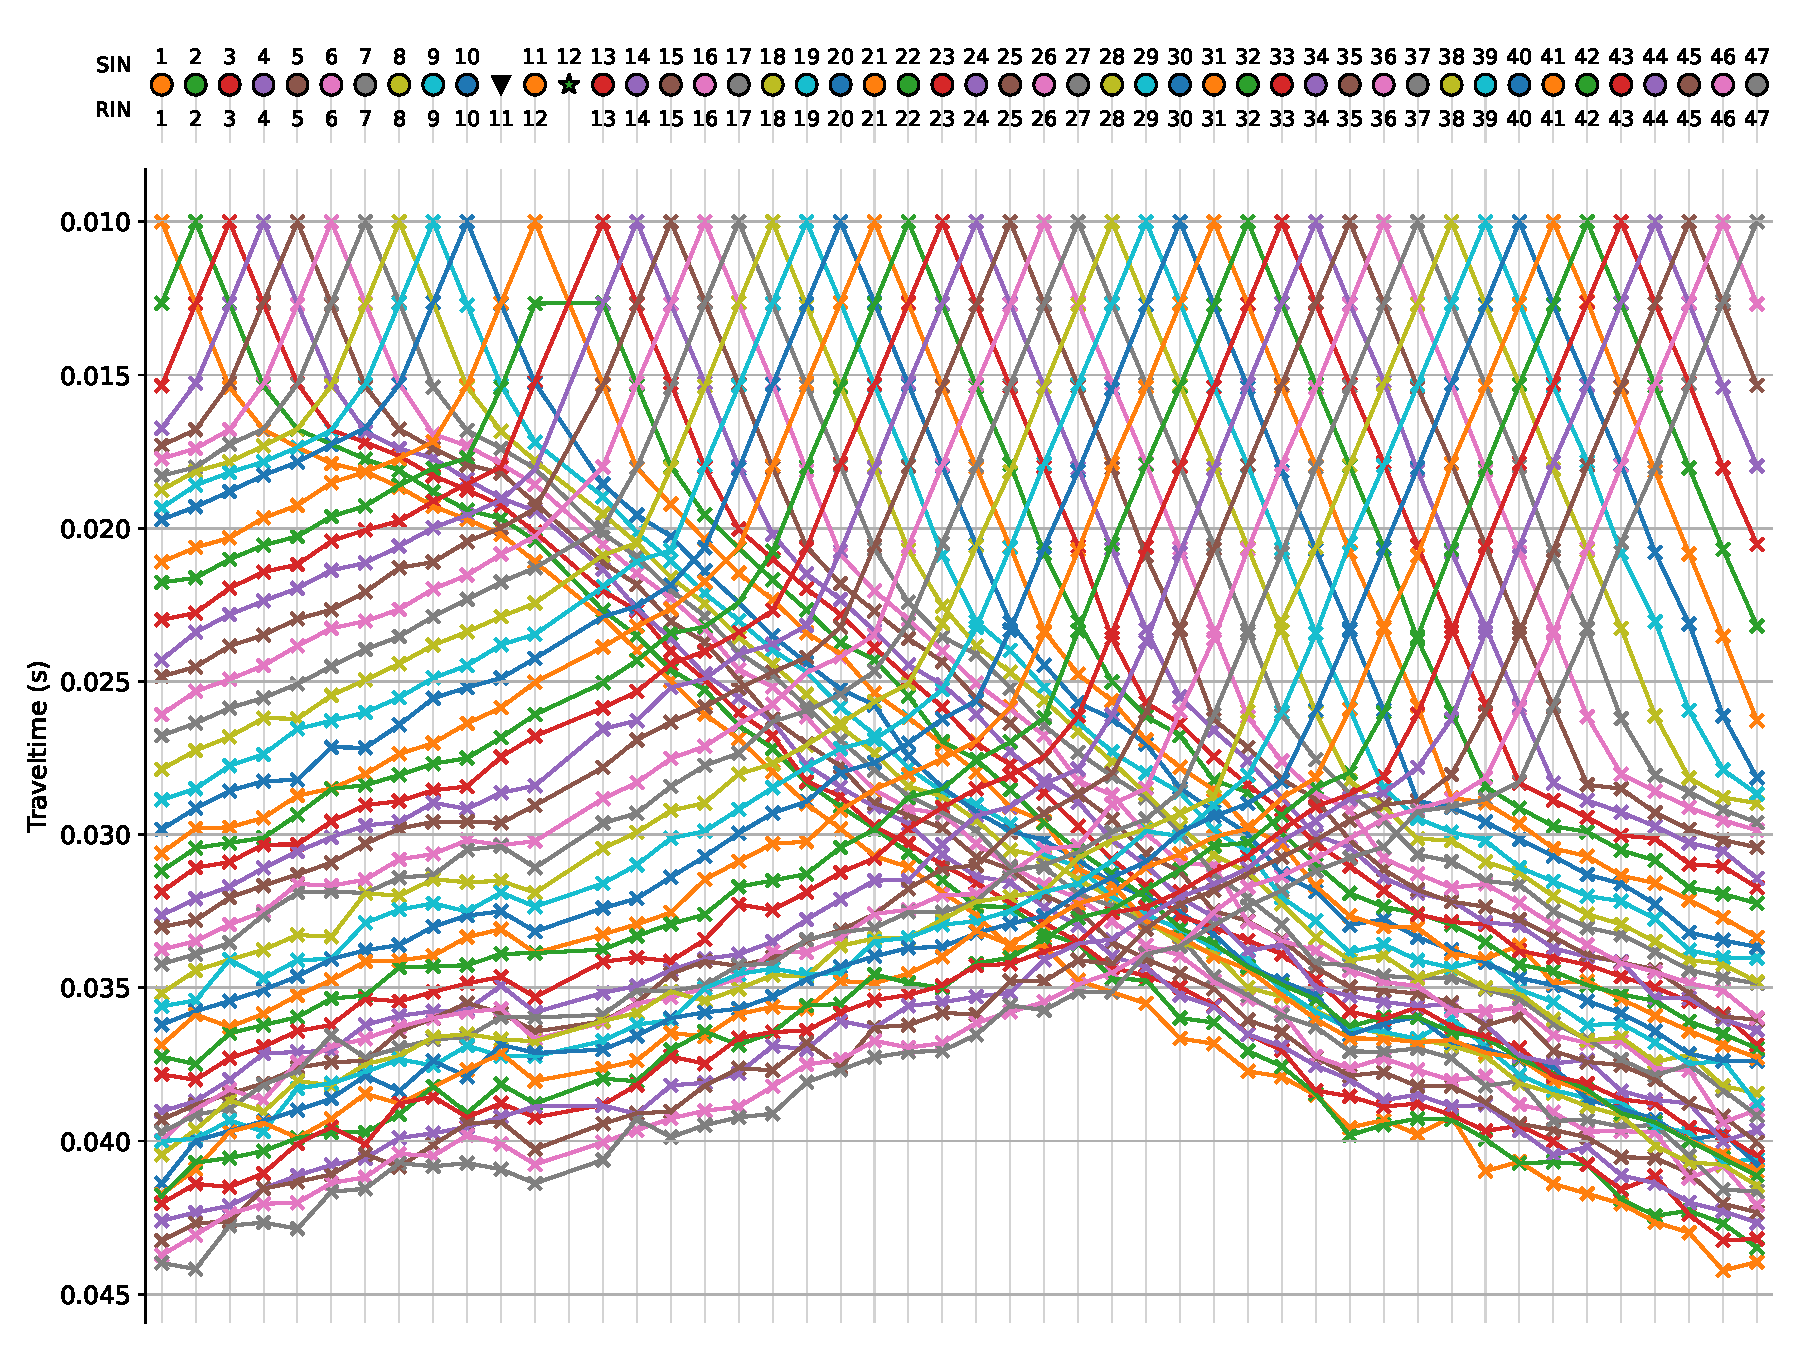
\includegraphics[width=.75\textwidth]{figures/traveltimes_syn.pdf}
	\caption{The traveltime diagram shows the first break traveltimes stored in the currently active pickset along the y axis (x symbols), where solid lines connect traveltimes assigned to a common shot. The sort order of the stations along the x axis reflects the geometry. Filled circles indicate stations with co-located shot and geophone (receiver), triangles refer to receiver stations (no shot) and stars refer to shot stations (no geophone).}
	\label{fig:traveltimes_intro}
\end{figure}
Once the user is satisfied with the quality of the first break traveltimes, the data points of the pickset can be exported in the unified data format, which is compatible with the pyGIMLi framework. In particular, the udf file is stored in the subdirectory \textit{03\_proc/picks} with the current timestamp as suffix:
\begin{lstlisting}[language=Python, firstnumber=22]
# Export first break traveltimes
srm.picksets(do='export', name='pick')
\end{lstlisting}
\begin{footnotesize}
\begin{verbatim}
INFO    : Pickset 'pick' saved to pick_20230303T140447.pck'
\end{verbatim}
\end{footnotesize}

\subsection{Expanding the capabilities of the formikoj library}
Making the formikoj library publicly available under an open-source license 
allows the addition of supplementary functionalities tailored for the specific requirements of the users.
The concept of formikoj suggest that such custom extensions should be implemented either as internal methods or as functions in the utilities module, which are then executed through the \texttt{compute} method.

We illustrate this possibility for customization by implementing a simplified version of an automatic first break picking algorithm based on the short- and long-time window average ratio (STA/LTA) method \citep{allen1978}, which determines the traveltimes following the energy ratio approach \citep[e.g.,][]{earle1994}. In particular, our implementation computes the envelope $E\left(t\right)$ of the seismogram $s\left(t\right)$ as \citep[e.g.,][]{duan2020}

\begin{equation}
	E(t)=\left(s\left(t\right)^2+\tilde{s}\left(t\right)\right)^{1/2}\,,
	\label{eq:envelope}
\end{equation}
where $\tilde{s}\left(t\right)$ is the Hilbert transform of $s\left(t\right)$. The energy ratio $ER$ is then computed as $ER=STA/LTA$ with

\begin{equation}
	STA\left(i\right)=\frac{1}{n_{STA}}\sum_{j=i-n_{STA}}^{i}E\left(j\right)\,,
	\label{eq:sta}
\end{equation}
and 

\begin{equation}
	LTA\left(i\right)=\frac{1}{n_{LTA}}\sum_{j=i-n_{STA}}^{i}E\left(j\right)\,,
	\label{eq:lta}
\end{equation}
where $n_{STA}$ and $n_{LTA}$ refer to the number of data points in $E\left(t\right)$ considered for the short- and long-time windows, respectively. For this exemplary implementation we determine the first break traveltimes in the seismograms as the position of the maximum in the $ER$ function, which is automatically saved in the project database. 

The autopicking algorithm is added to the \texttt{SeismicRefractionManager} in form of two internal methods\\ \texttt{\_manage\_autopicking} and \texttt{\_compute\_autopicks}, respectively. To invoke the autopicking process we modified the \texttt{compute} method, which now accepts the custom-defined keyword \texttt{autopicking}. Additionally, the autopicking requires values to be passed for the parameters \texttt{pick} and \texttt{pickset}. The former accepts the values \texttt{all} or \texttt{cur} to determine first break traveltimes for all traces in the dataset or solely the currently selected traces, respectively. The latter defines the name of the picksets in which the automatically determined traveltimes should be saved to. A typical use case involves conducting the autopicking and exporting the determined traveltimes:
\begin{lstlisting}[language=Python, firstnumber=24]
# Automatically pick first break traveltimes
srm.compute(do='autopicking', pick='all', pickset='autopicks')
srm.picksets(do='export', name='autopicks')
\end{lstlisting}
\begin{footnotesize}
\begin{verbatim}
INFO    : Created new pickset 'autopicks'
INFO    : Pickset 'autopicks' loaded
INFO    : 'autopicks' set at active pickset
Progress <==============================> 100.0% completed
INFO    : Pickset 'autopicks' saved to autopicks_20230303T140834.pck
\end{verbatim}
\end{footnotesize}

In Figure~\ref{fig:pickcomp}, we compare the automatically determined first break picks with the forward modeled traveltimes computed above to allow for a basic evaluation of autopicking performance. The inset plot in Figure~\ref{fig:pickcomp} presents the histogram of the autopicked traveltimes, which shows that three traveltimes should be considered outliers, and thus are removed from the dataset. After the outlier removal the correlation coefficient between forward modeled and autopicked traveltimes is \num{0.99} suggesting that the implemented autopicking algorithm performs well for the synthetic seismic waveform data. However, the observed deviation from the perfect correlation (i.e., the 1:1 line in Figure~\ref{fig:pickcomp}) indicates that autopicking and forward modeling algorithm might be sensitive to different seismic wave phases. Further improvements in terms of the autopicking process could incorporate, for example, machine learning approaches as the method proposed by \citet{duan2020}, which can be easily implemented as an additional functionality in the \texttt{SeismicRefractionManager}. We point out here, that following the same procedure, the user can implement further autopicking algorithms as well as other data processing strategies and have a simple framework for the evaluation of their performance through the analysis of synthetic data (e.g., clean and contaminated with Gaussian noise).
\begin{figure}
	\centering
	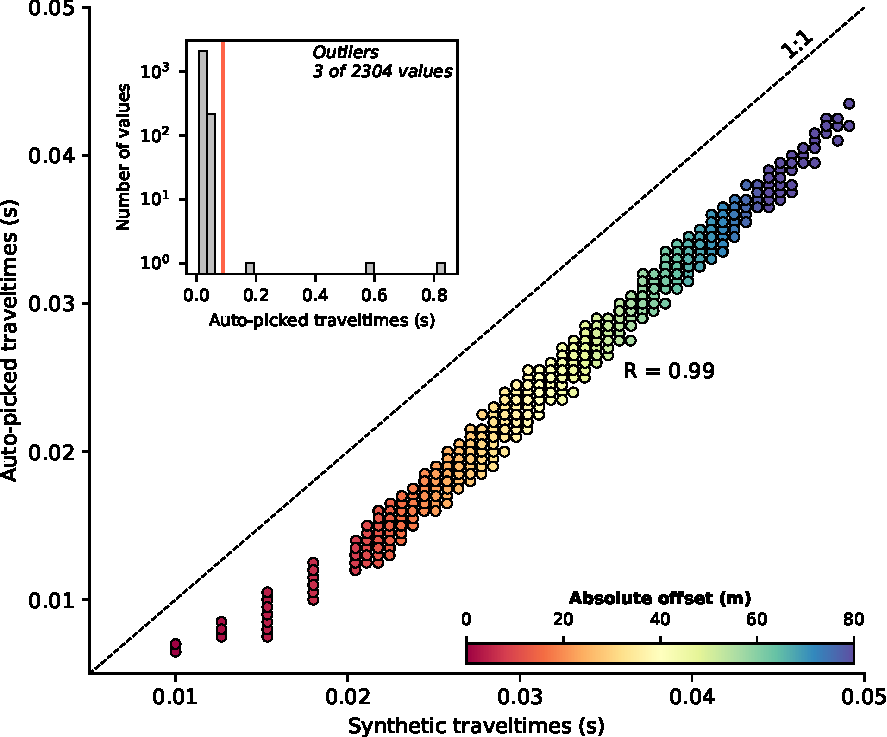
\includegraphics[width=.75\textwidth]{figures/pick_comparison.pdf}
	\caption{Comparison of forward modeled synthetic and automatically picked first break traveltimes for the synthetic seismic waveform data created in this study.}
	\label{fig:pickcomp}
\end{figure}

\section{Application to field data: Processing a 3D seismic refraction dataset}

To demonstrate the applicability of the  \texttt{SeismicRefractionManager} for the processing of real field data, we present here the analysis and inversion inversion results for a seismic refraction survey conducted in a soda lake located in the Nationalpark Neusiedler See--Seewinkel close to Vienna.
The seismic survey aims at solving for the geometry of the confined aquifer below this soda lake with the required information referring to the thickness of the aquifer and the depth of the groundwater table.
As presented in Figure~\ref{fig:map_sodalakes}, the seismic data were collected with 48 geophones deployed along the North-East to South-West oriented line, and 48 geophones along the North-West to South-East oriented line, with a spacing of \qty{2}{m} between the geophones. Shots were generated with an \qty{8}{kg} sledgehammer at the geophone positions as well as at positions along the diagonals to obtain a sufficient coverage.

\begin{figure}
	\centering
	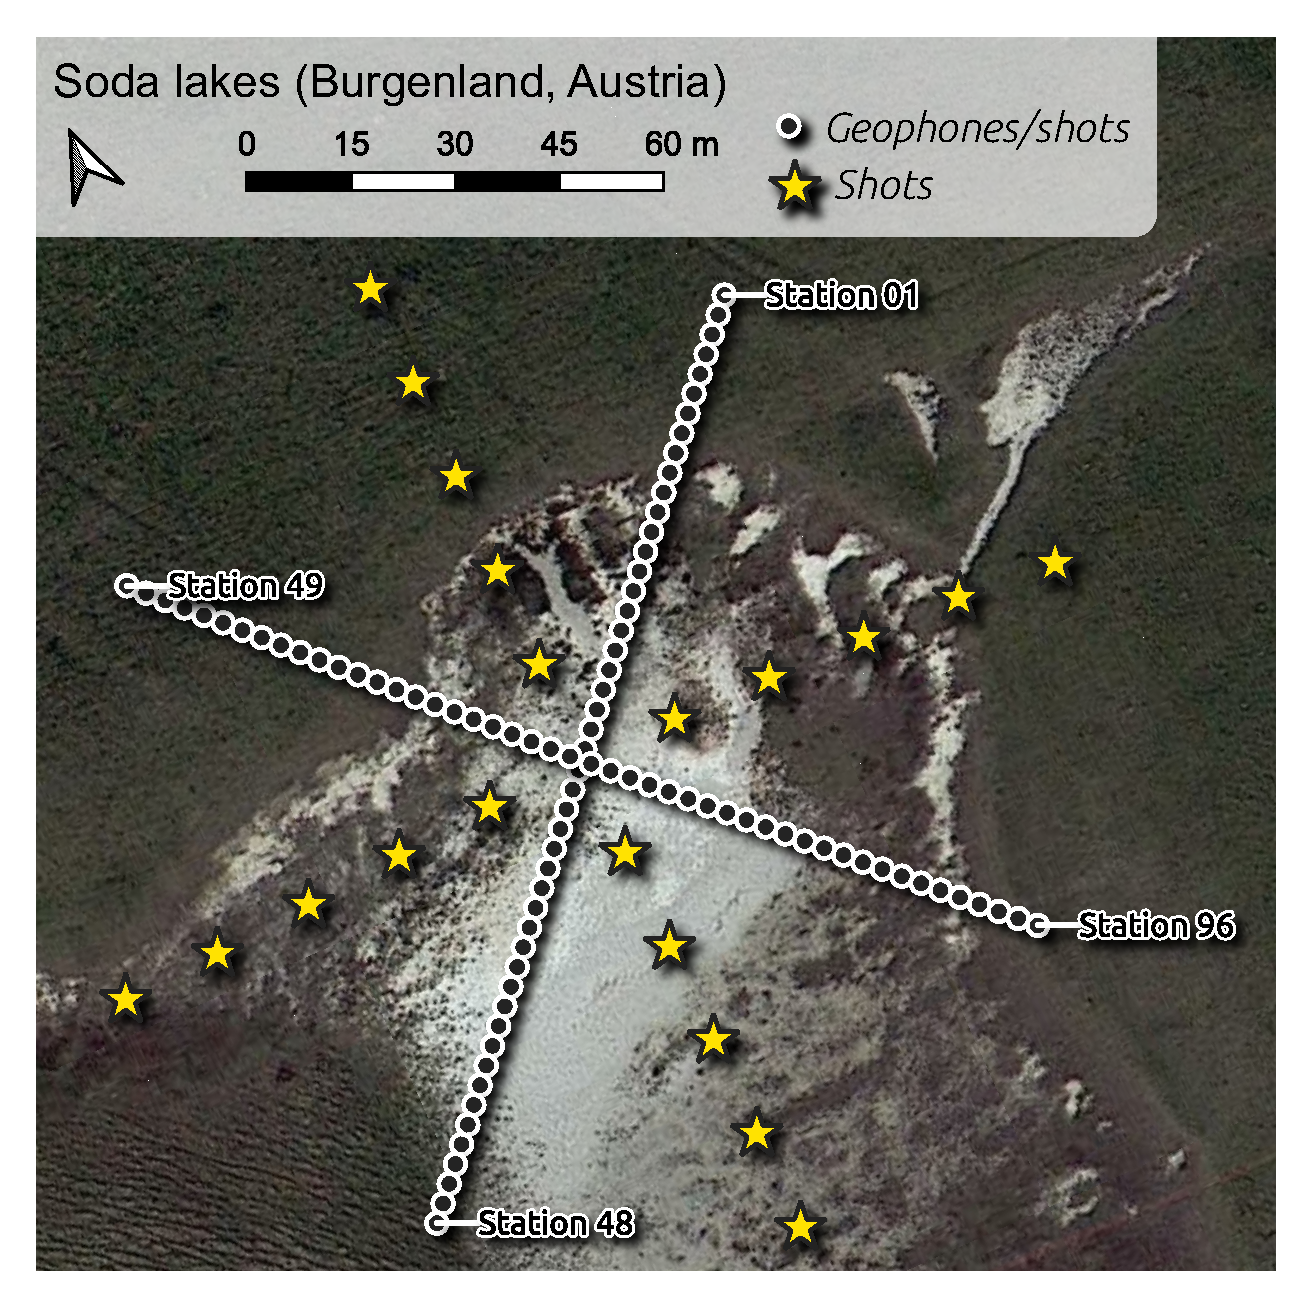
\includegraphics[width=.75\textwidth]{./figures/map_sodalakes.pdf}
	\caption{The soda lakes field dataset was collected in a 3D survey layout with stations (co-located geophones and shots indicated by filled dots) deployed in form of a cross. Additional shots (yellow stars) were conducted in from of a cross rotated by 45° to increase the coverage of the dataset.}
	\label{fig:map_sodalakes}
\end{figure}

As in case of the synthetic dataset presented above, the geometry file contains the coordinates of the survey stations, yet for the soda lake dataset 3D coordinates we provided as illustrated in Table~\ref{tab:3d_geometry}. 
Since geophones were not deployed at each survey station the column \textbf{Geo} contains the value 1 (True) for the first 96 stations and 0 (False) for the remaining \num{20} stations. 
\begin{table}
   \caption{Excerpt from the 3D survey geometry file.}
    \centering
    \begin{tabular}{rrrcrrr}
        \toprule
        \textbf{x (m)} & \textbf{y (m)} & \textbf{z (m)} & \textbf{Geo} & \textbf{Shot} & \textbf{1st Geo} & \textbf{\# Geo} \\
        \midrule
        40336.056 & 292470.692 & 120.0 & 1 & 1001	 & 1 & 96 \\
        40334.751 & 292469.177 & 120.0 & 1 & 1002 & 	1 & 96 \\
        \vdots & \vdots & \vdots & \vdots & \vdots & \vdots & \vdots \\
		40284.472 & 292455.431 & 120.0 & 1 & 1058 & 1 & 96 \\
		40285.896 & 292454.027 & 120.0 & 1 & 1059 & 1 & 96 \\
        \vdots & \vdots & \vdots & \vdots & \vdots & \vdots & \vdots \\
        40339.421 & 292402.681 & 120.0 & 1 & 1096 & 1 & 96 \\
		40305.228 & 292445.050 & 120.0 & 0 & 1097 & 1 & 96 \\
        \vdots & \vdots & \vdots & \vdots & \vdots & \vdots & \vdots \\
        40265.415 & 292431.957 & 120.0 & 0 & 1115 & 1 & 96 \\
		40255.453 & 292431.395 & 120.0 & 0 & 1116 & 1 & 96 \\
        \bottomrule
    \end{tabular}
    \label{tab:3d_geometry}
\end{table}
Based on the shot files and the geometry file stored in the required directory structure the \texttt{SeismicRefractionManager} creates the project database, automatically infers the 3D survey layout from the 3D survey geometry, and thus configures the project for 3D processing. Then we can select seismograms the same way as for the synthetic data presented above. For this example we select seismic waveform data recorded for SIN 1, i.e., the shot position co-located with the first geophone (Station 01 in Figure~\ref{fig:map_sodalakes}):
\begin{lstlisting}[language=Python, firstnumber=10]
# Select traces with receiver
srm.select(by='sin', num=1)
\end{lstlisting}
\begin{footnotesize}
\begin{verbatim}
INFO    : 96 traces selected
\end{verbatim}
\end{footnotesize}
In Figure~\ref{fig:3d_pickwindow}, we can see that the data for RIN 1 to 48 appear familiar as the corresponding SIN-RIN layout refers to the one of conventional 2D profiles; whereas the seismic waveforms for RIN 49 to 96 show an entirely different pattern. To understand such visualization, we need to take into account that RIN 49 to 96 are deployed perpendicular to the direction of propagation of the wavefront originating from SIN 1. Accordingly, the observed curvature in the first onsets is due to the varying offset of the different SIN-RIN pairs.
\begin{figure}
	\centering
	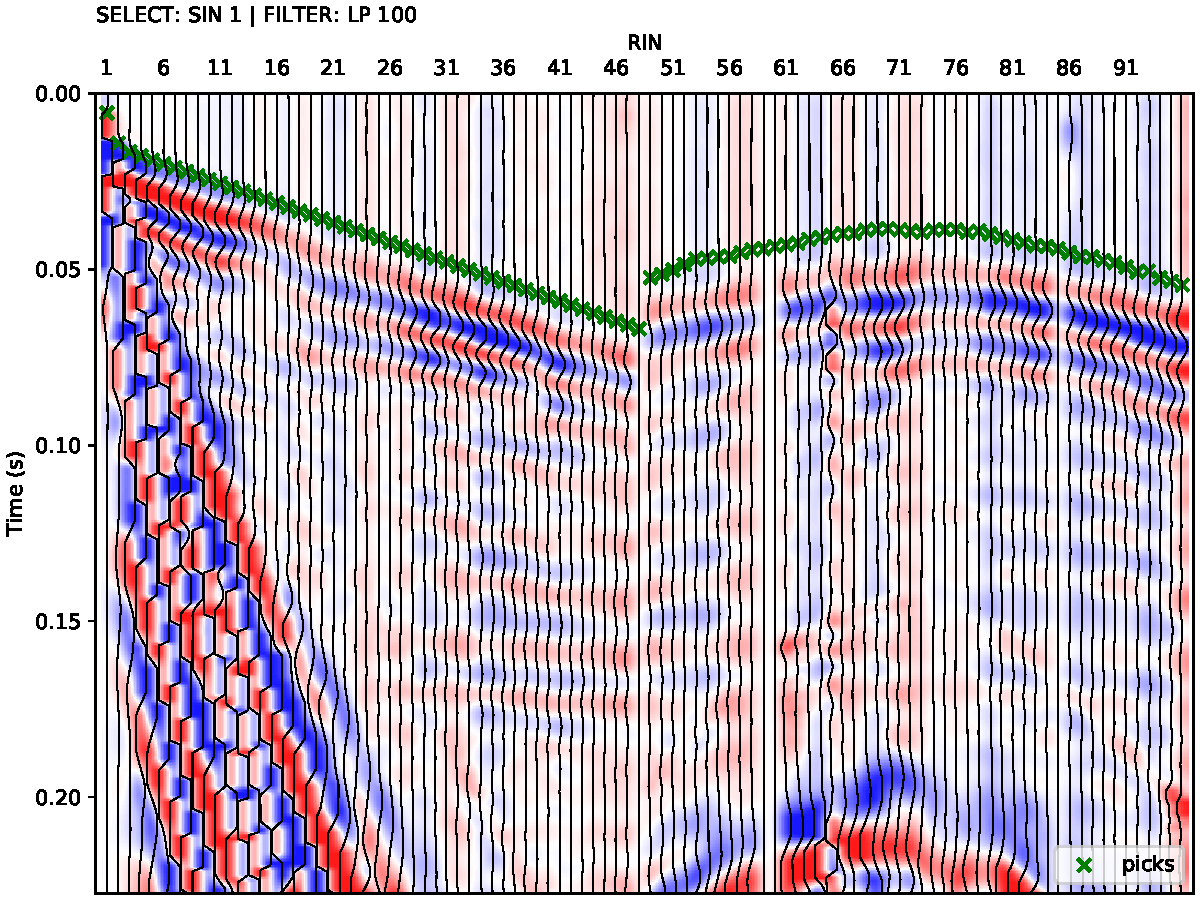
\includegraphics[width=.75\textwidth]{figures/sodalakes_sin1_lp100_picks_vd.pdf}
	\caption{Examplary seismic waveforms from the soda lakes dataset shown for shot index number (SIN) 1 with a 100 Hz lowpass filter applied to suppress high frequency noise. The recorded seismic waveforms clearly reflect the geometry of the geophones with RIN 1 to 48 deployed along the direction of wave propagation, while RIN 49 to 96 are deployed perpendicular to the propagating wavefront.}
	\label{fig:3d_pickwindow}
\end{figure}

Due to the 3D survey geometry, a 2D pseudosection is not suitable for assessing the quality of the first break traveltimes. However, the \texttt{SeismicRefractionManager} project is configured for 3D processing, and thus the apparent velocity values are illustrated in an interactive 3D pseudosection. This plot can be rotated and the image section can be zoomed and panned allowing the user to easily investigate the data quality for 3D geometries. Figure~\ref{fig:3d_pseudosection} shows a screenshot of the 3D pseudosection for the salt lake dataset; yet, such screenshot cannot reveal the full capabilities implemented in the \texttt{SeismicRefractionManger} for the interactive analysis and visualization of 3D pseudosections.

\begin{figure}
	\centering
	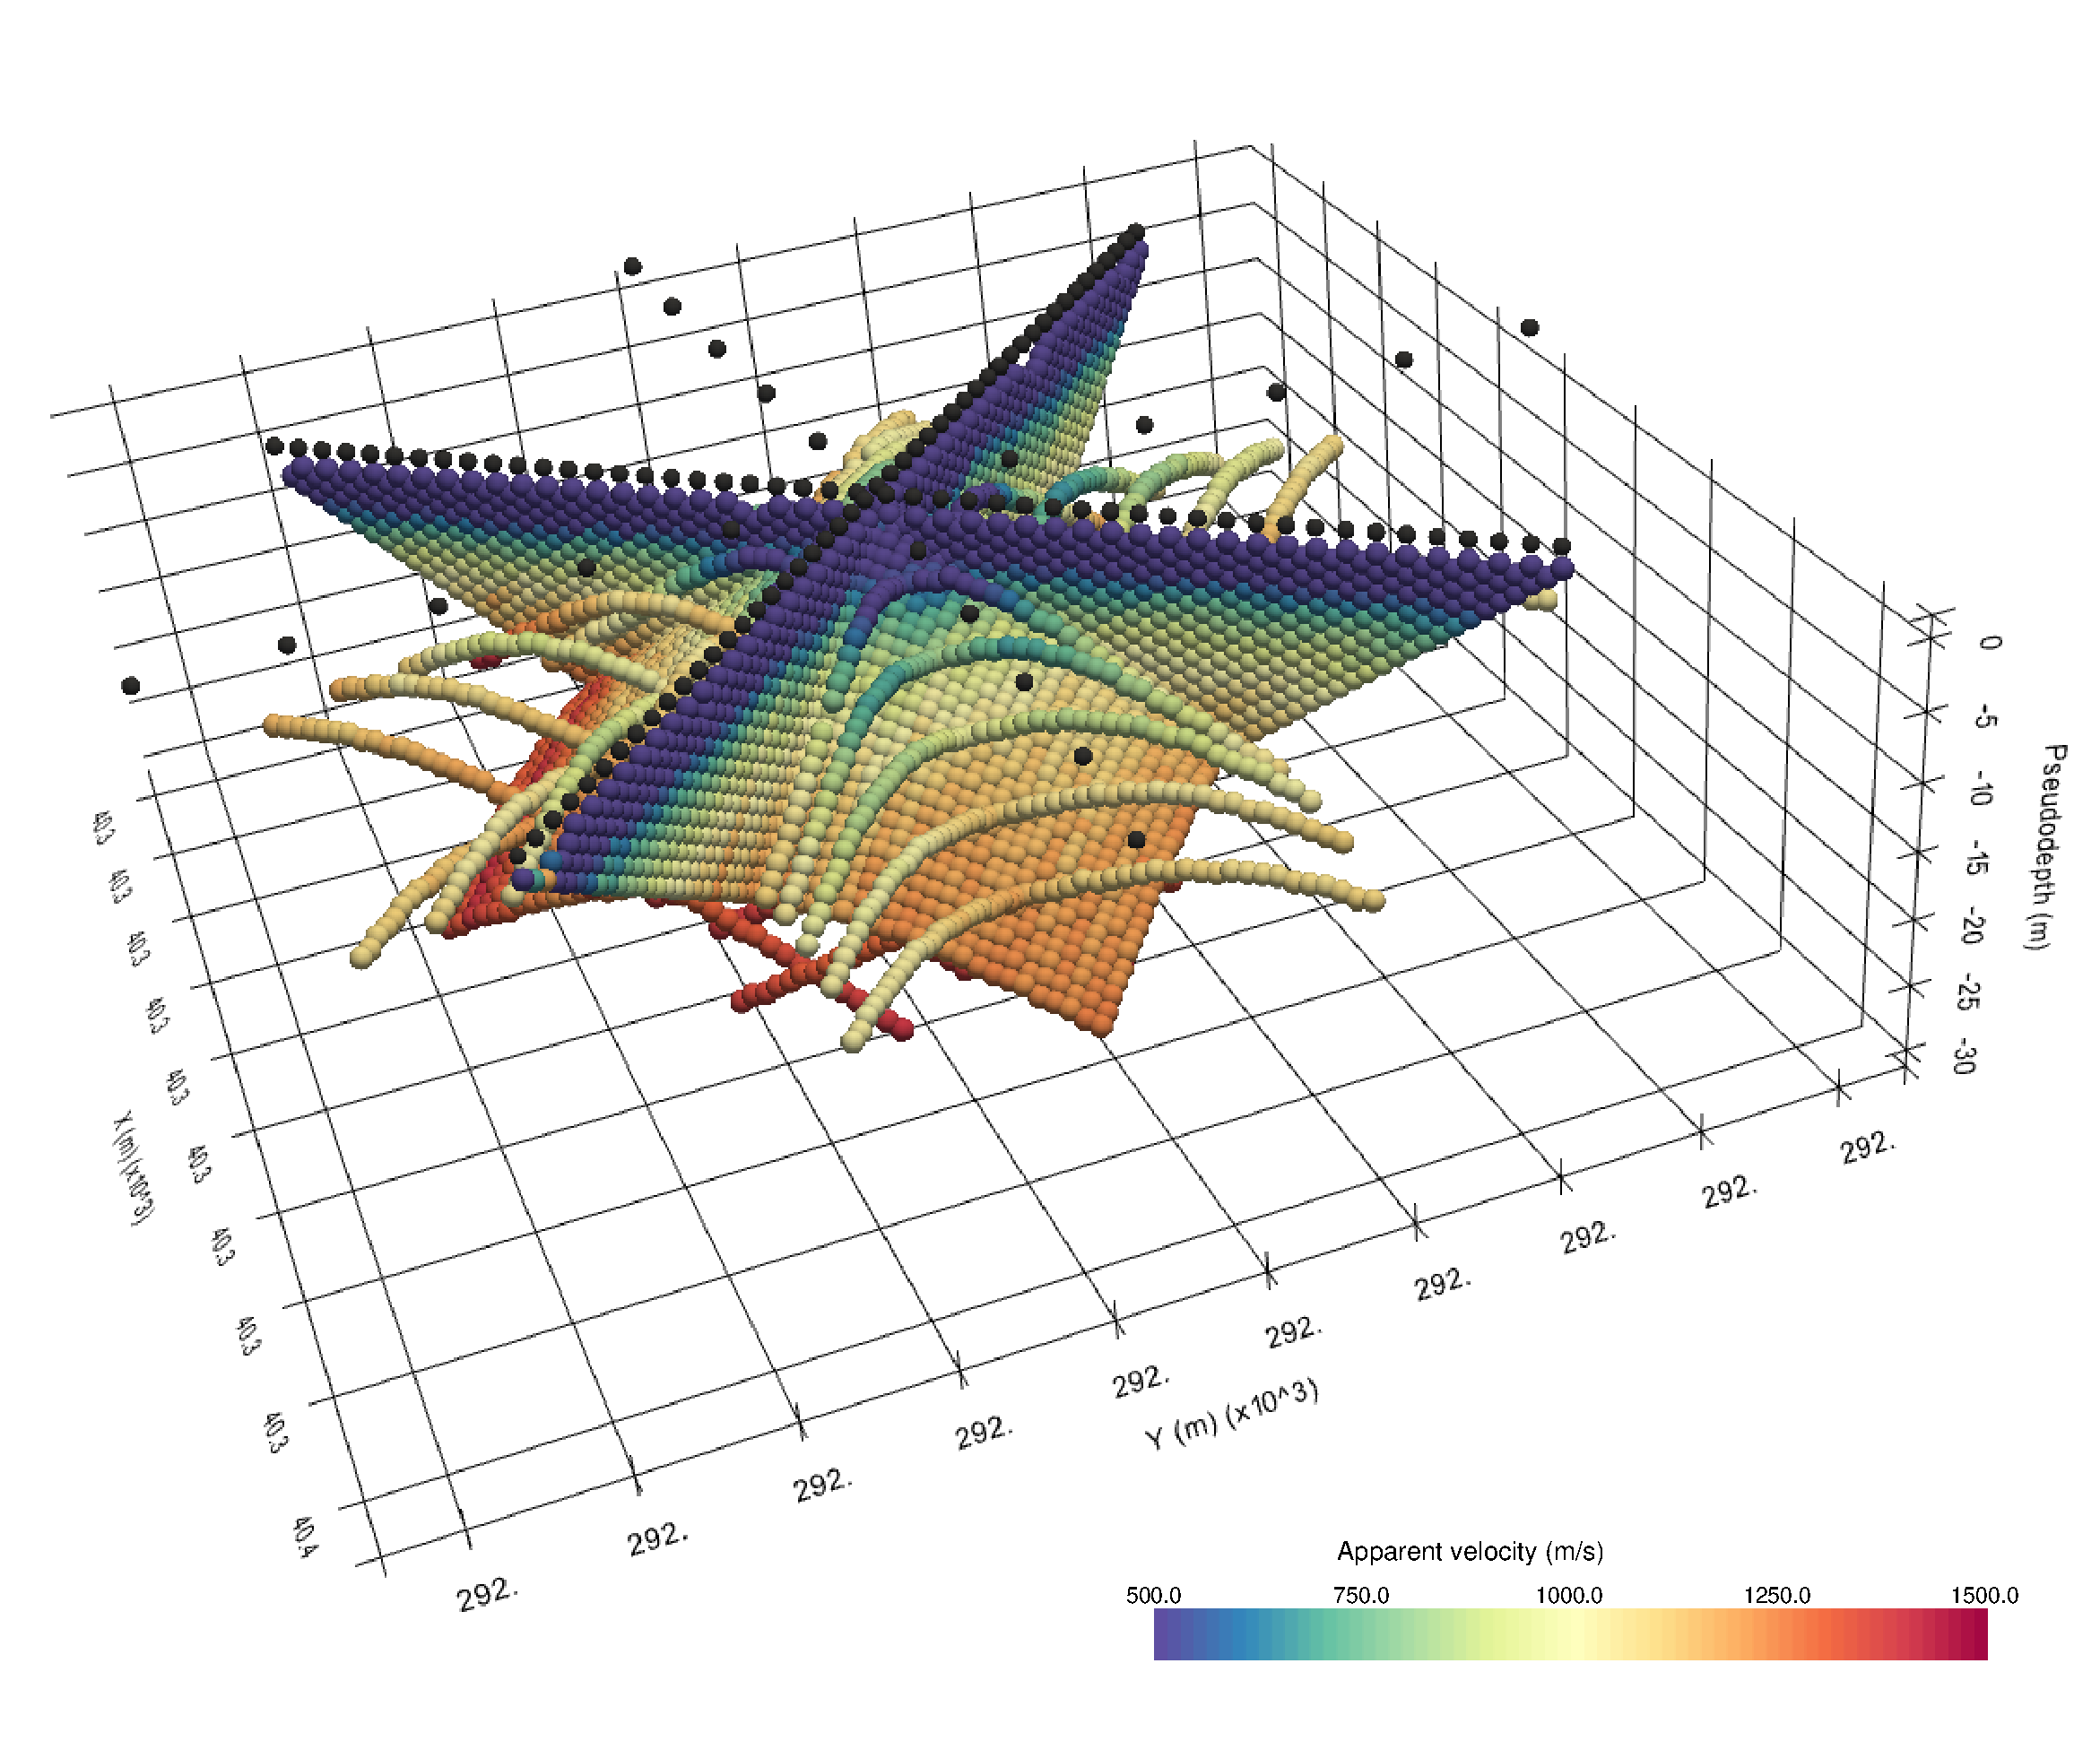
\includegraphics[width=.75\textwidth]{figures/3d_pseudosection.pdf}
	\caption{3D pseudosection showing the apparent seismic velocities determined from the first break traveltimes obtained from the soda lakes dataset and the corresponding absolute offset between the shot and receiver stations. The apparent velocity for each shot-receiver pair is illustrated at the corresponding 2D midpoint and pseudodepth (1/3 of the absolute offset), thus yielding a 3D representation.}
	\label{fig:3d_pseudosection}
\end{figure}

To review the data quality for the entire dataset it is possible to visualize the picking percentage, i.e., the ratio of actually picked traveltimes and total number of SIN-RIN pairs:
\begin{lstlisting}[language=Python, firstnumber=10]
# Plot the picking percentage
srm.plot(type='pickperc')
\end{lstlisting}
Figure~\ref{fig:3d_pickperc} presents the picking percentage visualized separately for each SIN. Accordingly, a low picking percentage indicates shots affected by a low signal-to-noise ratio, whereas clear first onsets yield a correspondingly high picking percentage. For the soda lake dataset we observe a consistently high picking percentage for all shot positions; thus, indicating a good data quality.
Moreover, the picking percentage plot can be used to track the picking progress, for instance, in case the traveltimes cannot be determined in frame of one session or to identify single shots that might have been forgotten during the first break picking. Accordingly, it is advisable to check the picking percentage prior to exporting the traveltimes for the inversion.

\begin{figure}
	\centering
	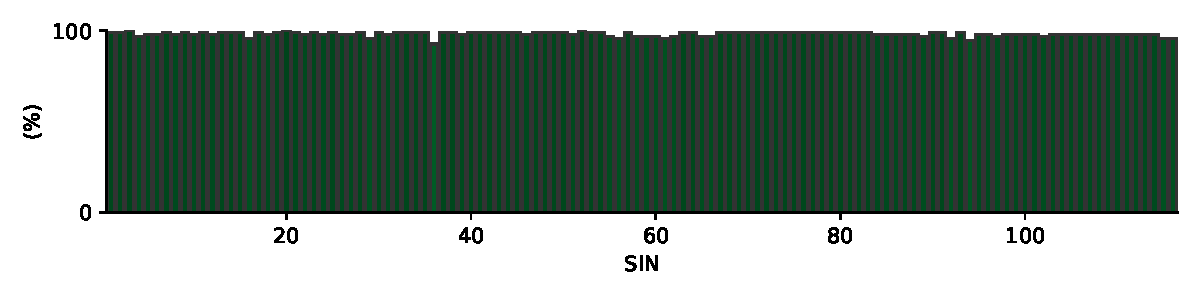
\includegraphics[width=.75\textwidth]{figures/3d_pickperc.pdf}
	\caption{Picking percentage for each shot in the soda lakes dataset indicating a high signal-to-noise ratio allowing for the picking of first break traveltimes for nearly all shot-receiver pairs.}
	\label{fig:3d_pickperc}
\end{figure}

Once the first break picking is finished, the corresponding pickset can be exported for the inversion. We inverted the first break traveltimes with pyGIMLi and present the resolved 3D subsurface model in Figure~\ref{fig:3dinvres}a. From this representation we can see, that the inversion solves for low seismic velocities (\num{600} to \qty{800}{ms^{-1}}) in the near-surface in the center of the investigated area, which corresponds to the still intact part of the soda lake, i.e., the part that is covered by water on a seasonal basis. Seismic velocity values above \qty{800}{ms^{-1}} are resolved at depth as well as outside of the soda lake.
To facilitate the interpretation of the resolved seismic velocity distribution in terms of the aquifer geometry we show the two vertical slices in Figure~\ref{fig:3dinvres}b and c, respectively. In particular, we relate seismic velocity values $>\,$\qty{800}{ms^{-1}} to the transition from the unsaturated to the saturated zone due to the higher seismic velocity of water ($\approx\,$\qty{1500}{ms^{-1}}) compared to air ($\approx\,$\qty{340}{ms^{-1}}) filling the pore space. Accordingly, our 3D subsurface model indicates the depth of the groundwater table at a depth of approximately \qty{8}{m}. A more detailed interpretation is beyond the scope of this manuscript, yet the presented figures reveal the capabilities provided by the proposed framework for the visualization and processing of data collected in 3D survey geometries.

\begin{figure}
	\centering
	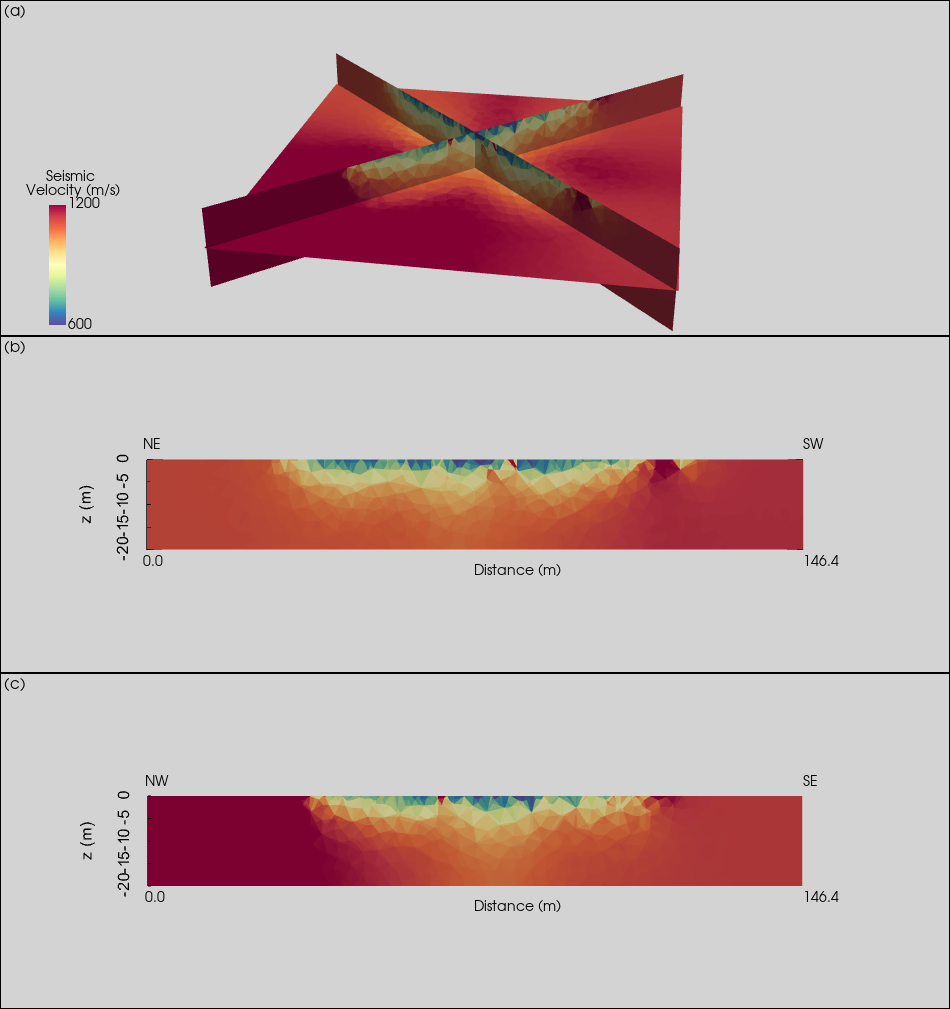
\includegraphics[width=.75\textwidth]{figures/inv_l100_ae0.0035.png}
	\caption{Subsurface model of the soda lake in terms of the seismic P-wave velocity. (a) 3D representation of orthogonal slices through the resolved subsurface model. (b) 2D representation of the NE--SW slice. (c) 2D representation of the NW--SE slice.}
	\label{fig:3dinvres}
\end{figure}

\section{Conclusions and Outlook}

We have presented formikoj, a flexible open-source library enabling the development of modeling and processing tools for geophysical data. Implemented in python and tested on all major operating systems (Linux/Unix, MacOS, Windows), formikoj is suitable for multi- and cross-platform applications; thus, allowing collaboration between users free from licensing costs and platform requirements.

We demonstrated the capabilities of the formikoj framework to develop versatile and easily scalable classes for the modeling and processing of waveforms in seismic refraction surveys. By standardizing the data input in combination with a thorough sanity check aims at reducing the risk of corrupting the information stored in the project database.
Moreover, crucial processing steps are automatized within the \texttt{SeismicWaveformModeler} and the\\ \texttt{SeismicRefractionManager} classes facilitated by efficient data input strategies, for instance the preparation and import of the geometry file or the keyboard-based interaction related to the first break picking. In this regard, the user controls the formikoj library by providing text-based commands preferably through an ipython shell to exploit the full interactive potential modeling and processing tools. However, applications of the formikoj library can also be automatized by implementing workflows in python scripts or jupyter notebooks.

By making the source code of the formikoj library available under the MIT license we intend to spark the development of further modeling and processing tools for various geophysical models based on this framework. Our further efforts will focus on implementing tools for other wave-based geophysical methods used in frame of our research activities, such as multi-channel analysis of (seismic) surface waves or magnetotelluric surveys. 

\section{Acknowledgments}

%The authors acknowledge TU Wien Bibliothek for financial support through its Open Access Funding Programme.
The authors are grateful to Nathalie Roser and Lukas Aigner for using and testing the formikoj library in frame of their research activities, and for providing valuable suggestions for improvement. Furthermore, we would like to thank Clemens Moser, Martin Mayr, Vinzenz Schichl and Harald Pammer for their constructive comments during first tests of the formikoj framework as well as for their help during the seismic surveys.

\newpage

\textbf{Code and data availability section}

Name of the code/library: formikoj

Contact: matthias.steiner@geo.tuwien.ac.at

Hardware requirements: No specific requirements

Program language: Python
 
Software required: Anaconda/Miniconda recommended

Total program and dataset size: 250 MB

The source codes and exemplary datasets are available for downloading at the link:

https://git.geo.tuwien.ac.at/msteine1/formikoj.git

The orthophoto used in Figure~\ref{fig:map_sodalakes} was published by geoland.at under a CC BY 4.0 license.

\appendix

\section{Source code for generating the subsurface model considered in this study}
\begin{lstlisting}[language=Python]
# Import required packages
import numpy as np
import pygimli as pg
import pygimli.meshtools as mt

# Create the model geometry
# - top layer
top = mt.createPolygon([[0, 0], [94, 0], 
                        [94, -3.5], [72, -3.5], 
                        [20, -2], [0, -2]],
                       isClosed=True, marker=1, area=0.1)

# - bottom layer
bottom = mt.createPolygon([[0, -2], [20, -2], 
                           [22, -6], [70, -6], 
                           [72, -3.5], [94, -3.5], 
                           [94, -10], [0, -10]],
                          isClosed=True, marker=3, area=0.1)

# - anomaly/infill
infill = mt.createPolygon([[20, -2], [72, -3.5], 
                           [70, -6], [22, -6]],
                          isClosed=True, marker=2, area=0.1)

geom = top + infill + bottom

# Define shot and receiver stations and create corresponding nodes
nstats = 48
spc = 2

stations = np.vstack((np.linspace(0, (nstats-1)*spc, nstats), 
                      np.zeros(nstats))).T

for p in stations:
    geom.createNode(p)

# Create mesh for the finite element modeling
mesh = mt.createMesh(geom, quality=34)

# Save the mesh in the binary mesh format for later use 
# with the SeismicWaveformModeler
mesh.save('mesh.bms')
\end{lstlisting}

\bibliographystyle{cas-model2-names}
\bibliography{references} 

\end{document}

